% NeuroCam manual - Top level
% Written by Christopher Thomas.
% Copyright (c) 2021 by Vanderbilt University. This work is released under
% the Creative Commons Attribution-ShareAlike 4.0 International License.

\documentclass[letterpaper,11pt]{report}
\usepackage[letterpaper]{geometry}
\usepackage{graphicx}
\usepackage{verbatim}

\geometry{nohead,footskip=0.3in,margin=0.75in}

% Force my paragraph style, darnit.
\usepackage{indentfirst}
\setlength{\parskip}{\baselineskip}

% Custom macros.
\newcommand{\fixme}[1]{\textbf{FIXME: #1}}

% Document body.
\begin{document}

% Title page.

\pagestyle{empty}

\begin{center}
%
\vspace*{1.5in}
{\Huge NeuroCam System Manual} \\
{\footnotesize Written by Christopher Thomas -- \today.} \\
%
\vspace*{1in}
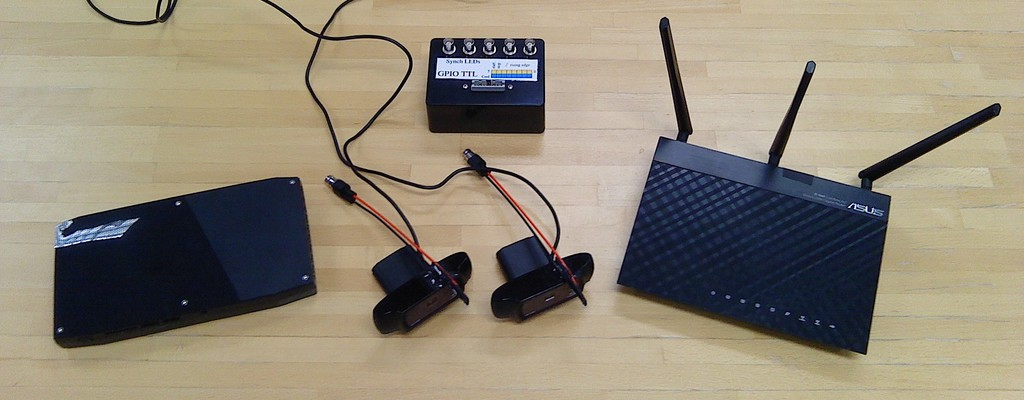
\includegraphics[width=0.9\textwidth]{pics-system/sys-all-d.jpg}
%
\vfill
{\footnotesize % NeuroCam manual - License tagline.
% Written by Christopher Thomas.
% Copyright (c) 2021 by Vanderbilt University. This work is released under
% the Creative Commons Attribution-ShareAlike 4.0 International License.
Copyright (c) \the\year\ by Vanderbilt University. This work is released under
the Creative Commons Attribution-ShareAlike 4.0 International License.
%
% This is the end of the file.
}
%
\end{center}
%
\clearpage
%
\pagestyle{plain}
\pagenumbering{roman}
\setcounter{page}{1}
%
\tableofcontents
%
\clearpage
\pagestyle{plain}
\setcounter{page}{1}
\pagenumbering{arabic}
% NOTE - "\thispagestyle" is used for part and chapter beginning pages,
% and overrides \pagestyle.
% Redefine it to be harmless.
% NOTE - The canonical solution ("\pagenumbering{gobble}") resets the page
% counter whenever it's used.
\renewcommand{\thispagestyle}[1]{}

% Part 1: User guide.

\clearpage
\pagestyle{empty}
\part{Using the NeuroCam System}
\pagestyle{plain}

% NeuroCam manual - Overview
% Written by Christopher Thomas.
% Copyright (c) 2021 by Vanderbilt University. This work is released under
% the Creative Commons Attribution-ShareAlike 4.0 International License.

\chapter{Overview}
\label{intro}

The NeuroCam system is a computer-controlled camera network that collects
footage of a subject interacting with a game (or other apparatus).
It was commissioned by the Attention Circuits Control Laboratory
(\verb+http://accl.psy.vanderbilt.edu/+)
to facilitate their experiments.

A system diagram is shown in Figure \ref{fig-system}, below:

\begin{figure}[h]
\begin{center}
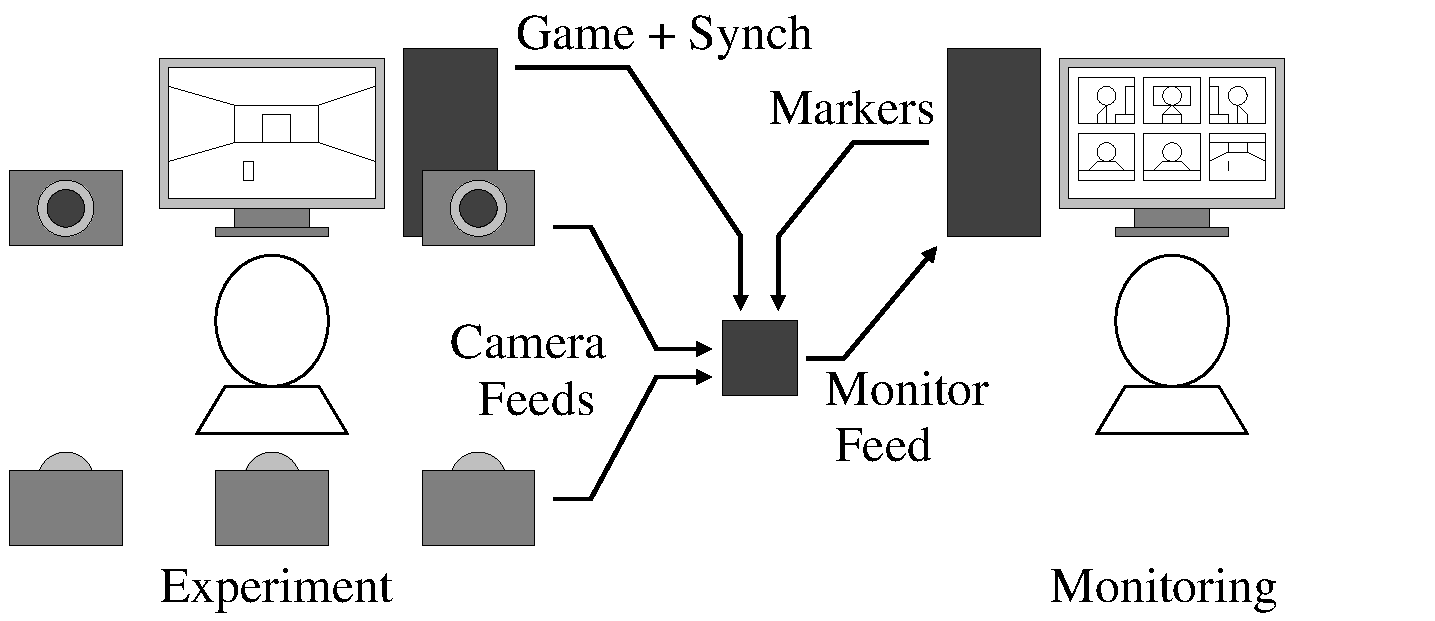
\includegraphics[width=0.95\textwidth]{figs/system-ext.pdf}
\end{center}
\caption{System block diagram.}\label{fig-system}
\end{figure}

The NeuroCam system processes several types of data and events (described
in detail in later sections):

\begin{itemize}

\item It collects frame data (with timestamps) from several cameras.

\item It collects streamed video data from the game machine.

\item It accepts web connections from authorized computers for control and
monitoring.

\item It provides a ``monitoring'' feed to the control computer showing
all video streams.

\item It records ``marker'' events when interface buttons are clicked on
the monitoring web page.

\item It records digital (TTL) signals from external equipment.

\item It accepts TTL ``start'' and ``stop'' signals from external equipment.

\item It offers collected data for examination, download, and
post-processing via a web interface after experiments have completed.

\end{itemize}

% NOTE - We can't mbox verbatim commands, so manually add line breaks.
To get started, connect an authorized machine to the ``\verb+neurocam+''
network and point it to \linebreak
``\verb+http://192.168.1.+\textit{(value)}''
(the IP address given on the sticker on the NeuroCam machine).

%
% This is the end of the file.

% NeuroCam manual - Hardware Setup
% Written by Christopher Thomas.
% Copyright (c) 2021 by Vanderbilt University. This work is released under
% the Creative Commons Attribution-ShareAlike 4.0 International License.

\chapter{Hardware Setup}
\label{setup}

The NeuroCam system has several hardware components:

\begin{itemize}

\item One ``NeuroCam'' embedded computer. This performs data collection and
storage.

\item One wireless router. This is connected to the NeuroCam computer and
to the game machine via wired LAN, and accepts wireless connections from
user machines. \textit{Do not connect this to the internet.}

The router used by the prototype system was an \mbox{Asus RT-N66U}.

\item One GPIO-and-synchronization box. This is connected to the NeuroCam
computer via USB, and provides TTL synchronization outputs over BNC and
accepts TTL-level inputs via a ribbon cable.

Any change in the TTL inputs is reported (and logged). A low-to-high
transition on bit 7 will start the NeuroCam recording, and a low-to-high
transition on bit 6 will stop recording (with a ``dead time'' of ten seconds
before further commands will be recognized). Input bits 0--5 are logged but
do not change NeuroCam behavior, and may be used for any desired purpose.

\item Five cameras, connected to the NeuroCam computer via USB.

The camera model used by the prototype system was the Logitech C920.

\end{itemize}

\begin{center}
% Black magic for the sizes here.
\begin{tabular}{cccc}
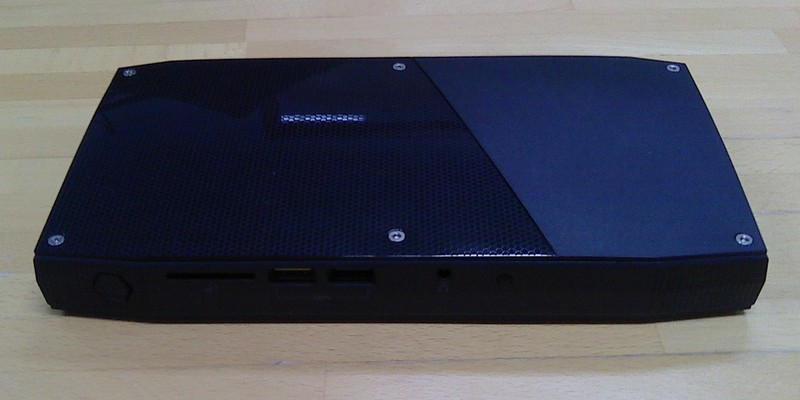
\includegraphics[height=0.14\textwidth]{pics-system/sys-comp-front.jpg} &
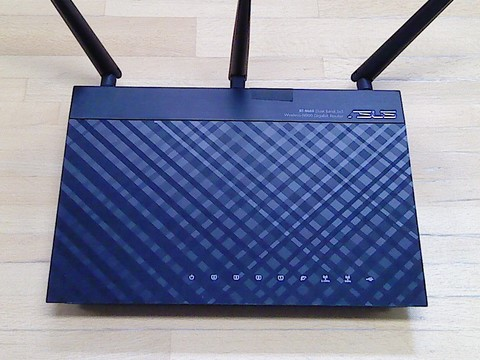
\includegraphics[height=0.14\textwidth]{pics-system/sys-router-front.jpg} &
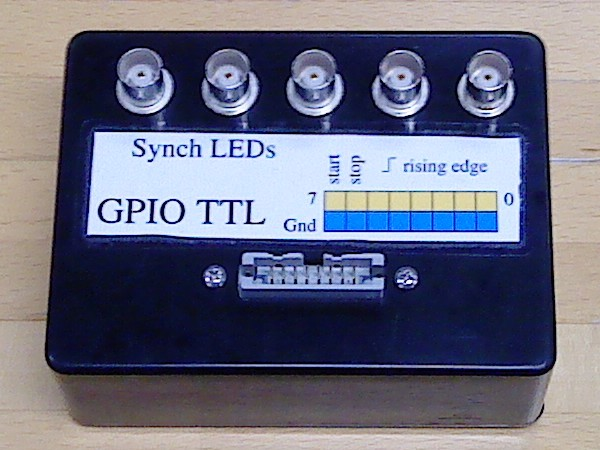
\includegraphics[height=0.14\textwidth]{pics-system/sys-gpio.jpg} &
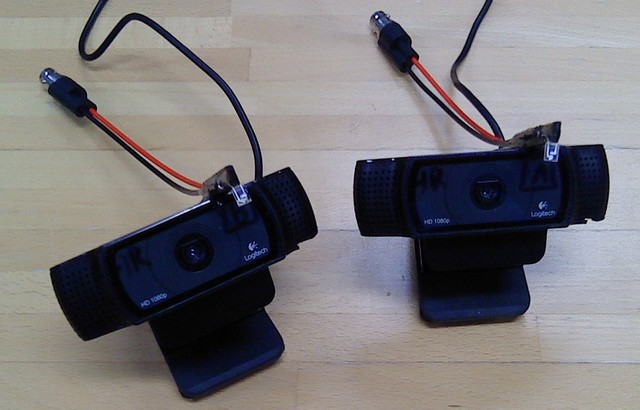
\includegraphics[height=0.14\textwidth]{pics-system/sys-cameras.jpg} \\
\end{tabular}
\end{center}

\clearpage

There are several tasks of note that have to be performed in order to
configure the NeuroCam hardware for use:

\begin{itemize}

\item The camera synchronization LEDs must be connected to the
GPIO-and-synchronization box via BNC cables.

Alternatively, a TTL-controlled lamp (visible or IR) may be placed in the
scene within view of all cameras and connected to the GPIO-and-synchronization
box.

\item The administrator password for the wireless router \textit{must} be
set to a new, stronger value. The default password (``administrator'') is
provided strictly for setup purposes.

The password for the NeuroCam network should also be changed. The default
password (``neurocam'') is easily guessed from the network name.

\item Any machines that are intended to communicate wirelessly with the
NeuroCam system must be added to the wireless router's MAC whitelist.
Machines that communicate via network cable may also need to be added,
depending on the router's configuration.

\item The game machine must be configured to stream MJPEG video, and to
respond to NeuroCam queries about offered content. The ``\verb+VLC+''
application was used for MJPEG streaming in the prototype system. Consult
VLC's documentation for further information.

Network handshaking with the game machine is described in Chapter 
\ref{handshake}.

\end{itemize}

The wireless router may be reconfigured by connecting to a wired LAN port
and accessing the web address printed on the bottom of the device.
\textbf{Do not} reset the device to factory default settings; this will lose 
all NeuroCam-related configuration.

See Chapter \ref{router} for details about configuring routers.

%
% This is the end of the file.

% NeuroCam manual - GUI
% Written by Christopher Thomas.
% Copyright (c) 2021 by Vanderbilt University. This work is released under
% the Creative Commons Attribution-ShareAlike 4.0 International License.

\chapter{Web Interface}
\label{gui}

The NeuroCam system has three interface screens: The \textbf{configuration}
screen, the \textbf{monitoring} screen, and the \textbf{repository browser}.
The monitoring screen is seen when the system is collecting data. When the
system is not collecting data, the configuration screen and the repository
browser are both available.

\textbf{Important:} Do not use the ``back'' button of your web browser to
switch pages. This will result in stale CGI information being submitted.
Use the navigation buttons in the NeuroCam application instead.

\section{Configuration Screen}
\label{gui-config}

\begin{figure}[h]
\begin{center}
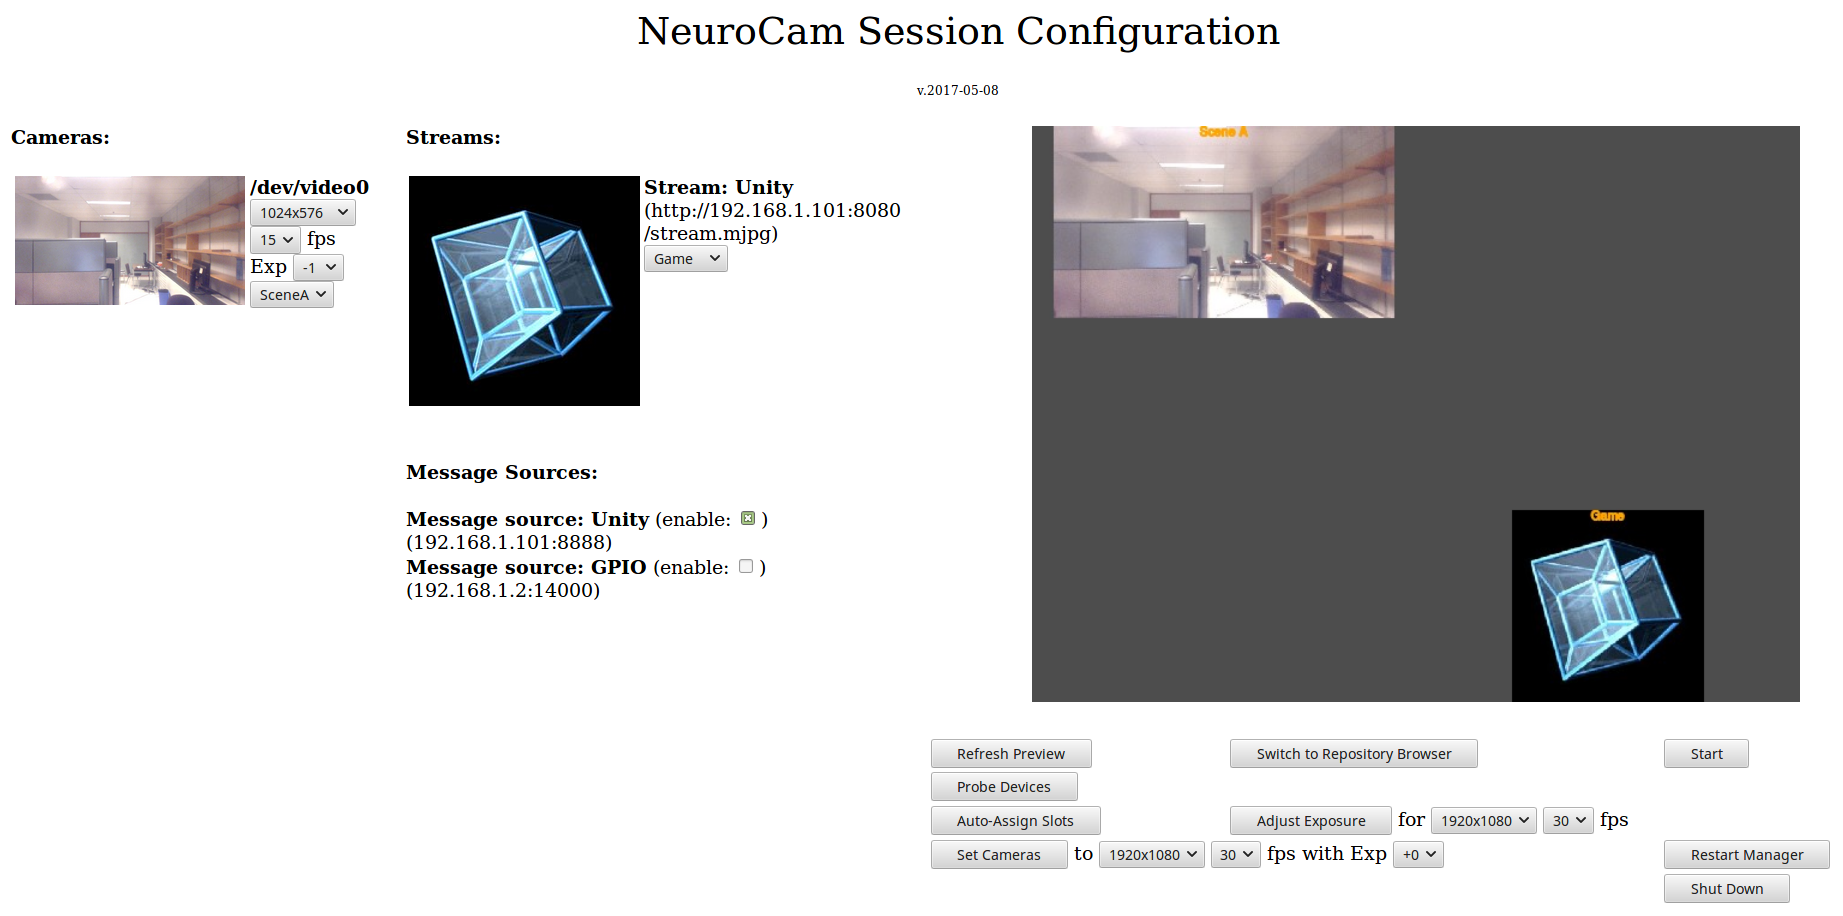
\includegraphics[width=0.95\textwidth]{pics-gui/gui-config.png}
\end{center}
\caption{Configuration screen.}\label{fig-gui-config}
\end{figure}

% FIXME - Annotate the image.

The configuration screen is used to set up a new video capture session.

Detected cameras are shown in the left column. The middle column shows
detected computer video streams and detected event message sources. The
right column shows a still-frame preview of the video feeds, with a control
panel under the preview.

Each camera has resolution, frame rate, and exposure settings, along with a
still-frame preview of its input. Longer (positive) exposures give a brighter
image but may reduce frame rate; shorter (negative) exposures give a dimmer
image but may increase frame rate. The ``slot'' to which the camera feed is
assigned may also be changed.

Camera settings may be changed all at once using the ``Set Cameras to...''
control in the control panel.

Camera settings may also be adjusted using the ``Adjust Exposure for...''
control in the control panel. This reduces exposure and resolution for each
camera until the specified frame rate is achieved. \textbf{Note:} this
adjustment takes several minutes (up to tens of minutes if the system has
difficulty finding appropriate settings).

There should always be at least one computer video stream, representing
a ``screencast'' of the game the subject is playing.

There should always be at least two event message sources: one from the game
computer (which sends game-time synchronization messages), and one from the
GPIO-and-synch box (which sends camera LED synchronization messages and
messages indicating changes in its TTL inputs).

The NeuroCam interface tries to enable appropriate message sources, choose
acceptable resolutions and frame rates, and assign appropriate feeds to
appropriate slots in the composite image, but some manual adjustment is
usually necessary. The ``Auto-Assign Slots'' control in the control panel
can be used to reset this assignment to the default.

The ``Refresh Preview'' button can be used to capture new images from the
cameras and computer video sources and to redraw the composite image preview.

\textbf{NOTE:} Some browsers may fail to update the preview images due to
cache behavior. Wait a moment and then click the ``preview'' button again
to refresh these images.

The ``Probe Devices'' button can be used to re-detect cameras, computer video
streams, and event/message feeds.

The ``Switch to Repository Browser'' button changes to the repository browser
screen, saving the configuration for later editing.

The ``Start'' button creates a new session directory, activates video capture,
and switches to the monitoring screen. This may alternatively be done by
raising the ``start capture'' TTL line.

The ``Restart Manager'' button forcibly restarts the NeuroCam software. This
allows recovery if any part of the NeuroCam software stops behaving correctly.
This is also needed if performing a software update without restarting the
NeuroCam machine.

The ``Shut Down'' button turns off the NeuroCam computer.

\section{Monitoring Screen}
\label{gui-monitor}

\begin{figure}[h]
\begin{center}
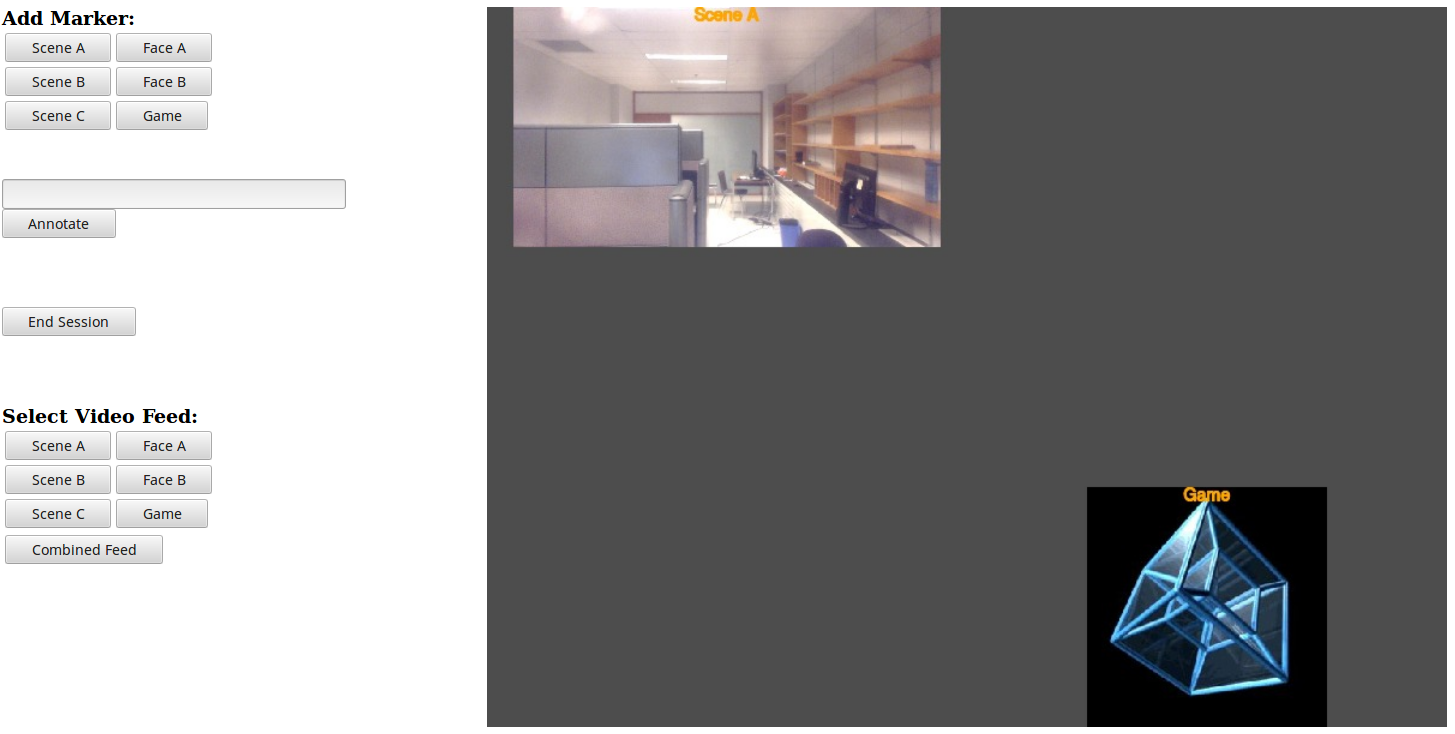
\includegraphics[width=0.95\textwidth]{pics-gui/gui-monitor.png}
\end{center}
\caption{Monitoring screen.}\label{fig-gui-monitor}
\end{figure}

% FIXME - Annotate the image.

The monitoring screen is used to view the progress of a capture session that
is underway, and to add event markers to the log file for this session.

The ``Add Marker'' buttons produce timestamped log entries indicating
events of interest in their respective video feeds.

The ``Annotate'' button produces a timestamped log entry containing
user-supplied text.

The ``End Session'' button stops video capture, closes the log file, and
switches to the repository browser screen. This may alternatively be done
by raising the ``stop capture'' TTL line.

The ``Select Video Feed'' buttons replace the combined image with the raw
video frames from the selected feed. This is usually better-quality and 
faster than the combined feed. The ``Combined Feed'' button returns to the
composite feed.

\section{Repository Browser}
\label{gui-repo}

\begin{figure}[h]
\begin{center}
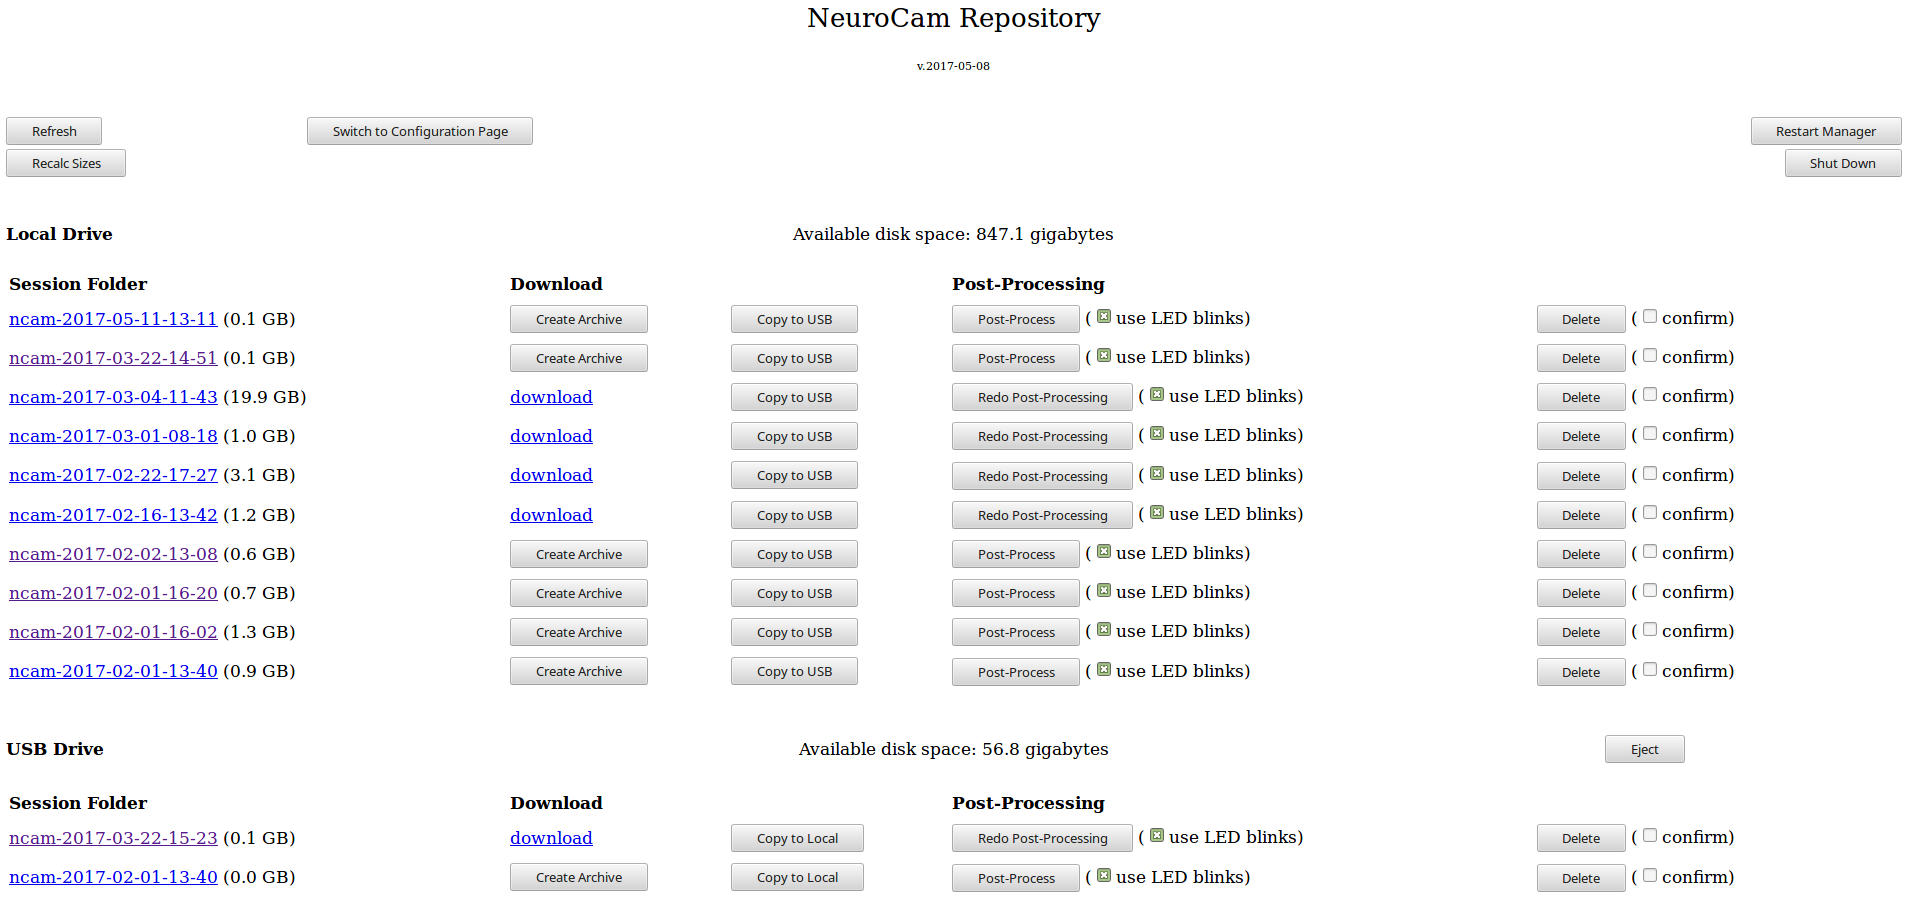
\includegraphics[width=0.95\textwidth]{pics-gui/gui-browser.png}
\end{center}
\caption{Repository browser.}\label{fig-gui-repo}
\end{figure}

% FIXME - Annotate the image.

The repository browser is used to inspect the data files produced by
past sessions, to perform post-processing of session data, and to download
and transfer packaged session data. Old sessions may also be deleted to free 
up disk space.

The ``Session Folder'' column lists sessions within the repository. Clicking
on a session name opens that session's directory in a new window. Files may
be individually inspected and downloaded via that window. See Chapter 
\ref{repo} for a description of the repository folder contents.

The ``Download'' column contains a link to a ``.tar'' archive containing
a session's entire directory tree. This is intended to provide an easy way
to transfer a session's data over the network. The archive is created using 
the ``Create Archive'' button. If post-processing has been performed, the 
archive includes the post-processed files. \textbf{NOTE:} The archive file 
is large. Check that there is sufficient free space before creating it.

The ``Copy to USB'' and ``Copy to Local'' buttons create duplicates of their
session folders on a USB-attached drive and on the local drive, respectively.
\textbf{NOTE:} These may instead be named ``Move to USB'' and ``Move to 
Local'', depending on settings. ``Move'' deletes the original folder, while
``Copy'' leaves it in place.

The ``Post-Processing'' button triggers several operations on a session 
folder. If the ``use LED blinks'' checkbox is set, video timestamps are
synchronized with each other using flashes of the infrared LEDs. A new log
file is saved with these adjusted timestamps. After synchronization, a
``Composite'' video feed is created, arranged in the same manner as the 
monitoring feed but at higher resolution and with full frame rate. A new log
file is saved with composite feed frame events added. Finally, movie files
of all video feeds are created for easy preview/playback.
\textbf{NOTE:} Post-processing operations take a lot of time on the local
drive (a solid-state drive), and even longer on magnetic platter or flash
drives.

\fixme{Benchmark post-processing. How long does processing an hour of
five-camera-plus-game footage take?}

The ``Delete'' buttons allow individual session folders (and their archives)
to be removed. This cannot be undone; to prevent accidental deletion, the
corresponding ``confirm'' checkbox must be checked before pressing the
``Delete'' button. Deleting old sessions will need to be performed frequently
in order to free up disk space.

The ``Eject'' button unmounts an external drive so that it can be safely
removed. \textbf{NOTE:} Writing data to an external drive can take a while,
so please wait until the NeuroCam indicates that it is safe for the drive
to be removed.

The ``Refresh'' button re-scans the repository directory for new sessions.

The ``Recalc Sizes'' button recomputes metadata for all session folders.
\textbf{NOTE:} This can take a while, as each session may contain millions
of files.

The ``Switch to Configuration Page'' button changes to the configuration
screen, so that the next capture session may be set up.

The ``Restart Manager'' button forcibly restarts the NeuroCam software. This
allows recovery if any part of the NeuroCam software stops behaving correctly.
This is also needed if performing a software update without restarting the
NeuroCam machine.

The ``Shut Down'' button turns off the NeuroCam computer.

%
% This is the end of the file.

% NeuroCam manual - Repository Data
% Written by Christopher Thomas.
% Copyright (c) 2021 by Vanderbilt University. This work is released under
% the Creative Commons Attribution-ShareAlike 4.0 International License.

\chapter{Repository Data}
\label{repo}

NeuroCam session data is stored in a ``repository''. Each session has its
own timestamped repository folder, containing some or all of the following:

\begin{itemize}

\item Raw video capture frames, stored as JPEG images in the ``Scene''
and ``Face'' folders.
\item Raw game capture frames, stored as JPEG images in the ``Game'' folder.

\item A ``Monitor'' folder containing reduced-size composited frames that
were sent to the monitoring GUI during the experiment. The composited frames
are not necessarily synchronized with each other.

\item A ``Composite'' folder containing larger composited frames produced
during post-processing. These composited frames should be synchronized.

\item A ``\verb+session.cfg+'' file containing information about the
settings used for the capture session. This file is described in detail in
Chapter \ref{structs}.

\item A ``\verb+logfile.txt+'' file containing raw event data (frame times,
user-supplied markers, and so forth).

\item Post-processed log files ``\verb+logfile-timed.txt+'' and
``\verb+logfile-composited.txt+''. The ``\verb+-timed+'' file has properly
synchronized timestamps and the ``\verb+-composited+'' file includes
timestamps for the ``Composite'' video stream (properly synchronized).

\item Several ``\verb+.mp4+'' compressed video files corresponding to the
video frame folders described above. These are lower-fidelity copies intended
to simplify review of footage.

\end{itemize}

% FIXME - Force a page break.
\clearpage
A typical session folder before post-processing is shown below:
\begin{center}
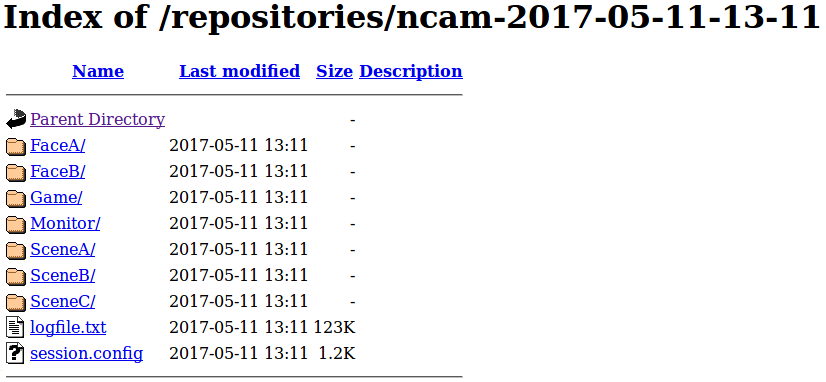
\includegraphics[width=0.6\textwidth]{pics-gui/gui-repo-unprocessed.png}
\end{center}

A typical session folder after post-processing is shown below:
\begin{center}
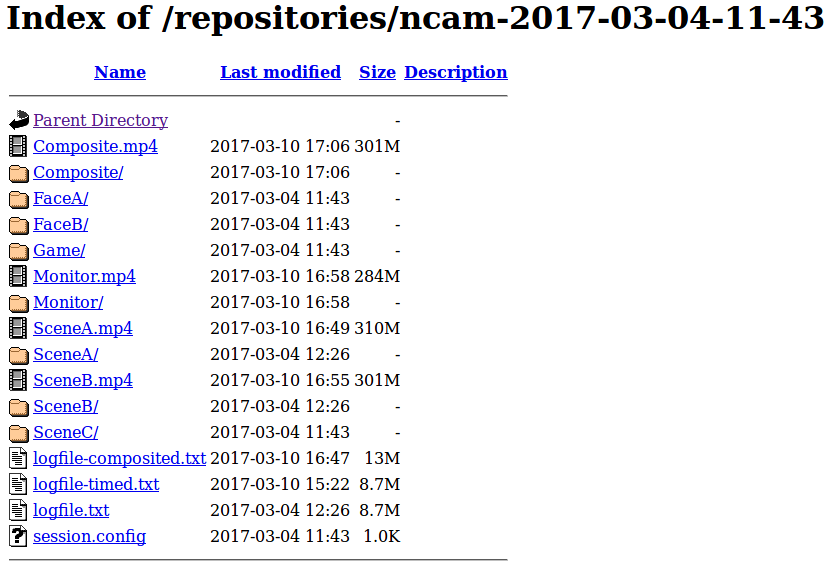
\includegraphics[width=0.6\textwidth]{pics-gui/gui-repo-afterprocess.png}
\end{center}

% FIXME - Force a page break.
\clearpage
\section{Log File Format}

The logfile is a human-readable text file recording one event per line. The 
following types of event are recorded:
\begin{itemize}
\item \textbf{Frame events}, indicating that a video frame was recorded.
This may be from a camera, from a remote computer video feed, or from a
generated feed like the ``Monitor'' and ``Composite'' feeds.
\item \textbf{Network message events}, which are typically sent by the
GPIO-and-synch box or by external applications such as the game.
\item \textbf{Local GUI events}, which are either user annotations, user
markers, or instructions to change the monitoring display.
\end{itemize}

\textbf{Frame events} indicate arrival time, stream ``slot'' name, sequence 
number, and the filename (including subfolder) where the frame was saved. 
Typical frame events are as follows:
\begin{verbatim}
(1367) [SceneA]  frame 8  SceneA/00000008.jpg
(1374) [SceneB]  frame 16  SceneB/00000016.jpg
(1382) [Monitor]  frame 36  Monitor/00000036.jpg
(1403) [SceneB]  frame 17  SceneB/00000017.jpg
(1417) [Monitor]  frame 37  Monitor/00000037.jpg
(1437) [SceneA]  frame 9  SceneA/00000009.jpg
(1444) [SceneB]  frame 18  SceneB/00000018.jpg
\end{verbatim}

\textbf{Netowrk events} indicate arrival time, IP and port of the source,
and a message string. Typical network events are as follows:
\begin{verbatim}
(304) [192.168.1.101:8888]  MSG Unity timestamp 53284 ms
(1303) [192.168.1.101:8888]  MSG Unity timestamp 54283 ms
(2303) [192.168.1.101:8888]  MSG Unity timestamp 55283 ms
(2795) [192.168.1.2:14000]  MSG gpio A0 O: 01
(2815) [192.168.1.2:14000]  MSG gpio A0 O: 00
(3303) [192.168.1.101:8888]  MSG Unity timestamp 56283 ms
(4303) [192.168.1.101:8888]  MSG Unity timestamp 57283 ms
\end{verbatim}

\textbf{Local GUI events} indicate event time, the fact that the event was
local, and a command, annotation, or marker string. Typical local events
are as follows:
\begin{verbatim}
(23197) [local]  CMD monitor SceneA
(39396) [local]  Marker: Game
(48249) [local]  CMD monitor Game
(76264) [local]  CMD monitor SceneA
(104119) [local]  CMD monitor Monitor
(491174) [local]  User annotation: "task started"
\end{verbatim}

%
% This is the end of the file.

% NeuroCam manual - Game Machine Handshaking
% Written by Christopher Thomas.
% Copyright (c) 2021 by Vanderbilt University. This work is released under
% the Creative Commons Attribution-ShareAlike 4.0 International License.

\chapter{Game Machine Handshaking}
\label{handshake}

The NeuroCam system queries machines on the local network to find content
providers. For the prototype system, the only network content provider is
the game machine.

The game machine should listen for UDP packets on port 8888. These will
be any of the following messages in plain text:
\begin{itemize}
\item ``\verb+looking for sources reply to port NNNN+''
\item ``\verb+talk to me on port NNNN+''
\item ``\verb+stop talking+''
\end{itemize}

The game machine may send any of the following responses:
\begin{itemize}
\item ``\verb+stream source at http://URL label XXXX+''
\item ``\verb+message source at HOST:PORT label XXXX+''
\item ``\verb+MSG (message text goes here)+''
\end{itemize}

The game machine will typically offer one video stream (the game video) and
one message source (which sends plain text timestamps for synchronization of
game events and NeuroCam data).

The video URL will generally be of the form
``\verb+http://(host IP):(port)/(file).mjpeg+''. Any valid URL should work,
as long as the file has the suffix ``\verb+mjpeg+'' and as long as the
host is given by IP address rather than hostname. This video stream will be
fetched by the NeuroCam and treated like any other camera feed.

Message sources must use IP addresses (not hostnames) as the host identifier.
These will be sent ``\verb+talk to me+'' and ``\verb+stop talking+''
messages, and when active are expected to send plain text UDP messages to
the NeuroCam machine. Messages are expected to begin with ``\verb+MSG +'',
with message content transcribed to the NeuroCam session log file. Message
source and NeuroCam timestamp information are also recorded in the log.

Multiple machines may respond to the broadcast query, and the same machine
may respond multiple times to one query. As long as the message and video
stream sources indicated by the responses are unique, they will all be
available to the NeuroCam system.

%
% This is the end of the file.


% Part 2: Maintenance guide.

\clearpage
\pagestyle{empty}
\part{Making More NeuroCam Systems}
\pagestyle{plain}

% NeuroCam manual - NeuroCam Computer
% Written by Christopher Thomas.
% Copyright (c) 2021 by Vanderbilt University. This work is released under
% the Creative Commons Attribution-ShareAlike 4.0 International License.

\chapter{NeuroCam Computer}
\label{machine}

The NeuroCam computer is a small--form--factor x86--architecture computer
running the Linux Mint operating system and the NeuroCam software.

To build a new NeuroCam computer, you will need the following:
\begin{itemize}
%
\item A suitable computer.
\item A USB stick containing the Linux Mint installer.
\item A USB stick containing the NeuroCam installer.
%
\end{itemize}

Details of the hardware and the installation process are described in their
appropriate sections. The procedure for making new USB sticks is also
described.

%
%
%
\section{Hardware}

The NeuroCam computer must be powerful enough to perform image compositing
in real-time, have a solid--state drive that is fast, large, and has high
endurance, and have enough RAM to handle any cacheing and buffering
transparently.

The components used for the NeuroCam prototype are as follows:

\begin{tabular}{llll}\hline
Qty & Description & Manuf. p/n & NewEgg SKU \\
\hline
%
1 & Intel NUC with Core i7 & Intel NUC6i7KYK & N82E16856102166 \\
% This is 1x 8 gig.
1 & DDR4 260-pin SO-DIMM 8G$^*$ & Ripjaws F4-2133C15S-8GRS & N82E16820232147 \\
% This is 2x 4 gig. We only _need_ 1x 4 gig.
%1 & DDR4 260-pin SO-DIMM 4G$^*$ & Ripjaws F4-2133C15D-8GRS & N82E16820232146 \\
1 & SSD 1 TB high-endurance M.2 & Samsung MZ-N5E1T0BW & N82E16820147567 \\
%
\hline
\multicolumn{4}{l}{$^*$A single 4-gig stick is sufficient, but no longer in
NewEgg's catalogue.} \\
\end{tabular}

To assemble the computer (Intel NUC version):
\begin{itemize}
%
\item Ensure that the workspace is free of clutter and clean.

\item Ensure that clothing is not carrying electrostatic charge. A humidifier
can reduce static electricity in the workspace if necessary.

\item Remove the skull-logo faceplate and set it aside. Unpack the plain
faceplate as a replacement.

\item With the machine interior exposed, carefully seat the RAM in the lower
DIMM slot. Apply \textbf{gentle} pressure until the latches engage to secure
the RAM. It may be necessary to open the latches by hand to fully insert the
RAM.

\item Remove the securing screw for the first solid-state drive slot, and
insert the solid-state drive. Ensure that the drive is seated firmly in its
connector, and reinstall the securing screw.

\item Reinstall the faceplate.
%
\end{itemize}

%
%
%
\section{Installing Mint and the NeuroCam Software}

The prototype NeuroCam machine used Linux Mint 18.1. This version or any later
version should have full driver support for the specific Intel NUC machine
described above.

You will need a Mint 18.1 install USB stick and a NeuroCam install USB stick.
Making these is described in Sections \ref{machine-usbmint} and
\ref{machine-usb}, respectively.

%
\subsection{First-Time Installation}

To install Linux and the NeuroCam software:
\begin{itemize}
%
\item Connect the machine to a keyboard, a mouse, and an HDMI monitor.
\item With the machine unpowered, plug in the Mint 18.1 USB stick.
\item Turn on the machine.
\item Hit F2 to get to the BIOS menu.
\item Turn UEFI off. This may be called ``Windows compatibility''.
\item Edit the boot order, moving the USB stick to the top.
\item Hit F10 to save and exit.
%
\item (The machine should now show the Linux boot menu.)
\item From the Linux boot menu, pick ``start in compatibility mode''.
\item From the GUI, open a terminal window.
\item Type ``\verb+sudo bash+'' to get a root session.
\item Type ``\verb+fdisk /dev/sda+'' to partition the solid--state drive.
\item Delete any existing partitions. The normally won't be any.
\item Create a 50 gigabyte partition (for the OS), an 8 gigabyte partition
(for swap space), and a third partition (for data).
\item Set the OS and data partitions to type 83 (Linux; this may be set
already by default). Set the swap partition to type 82 (Linux swap).
\item Set the ``bootable'' flag on the OS partition.
\item Save and exit \verb+fdisk+.
\item Type ``\verb+mke2fs -j /dev/sda1+'' and
``\verb+mke2fs -j -m 0 /dev/sda3+'' to create filesystems on the OS and
data partitions, respectively.
\item Type ``\verb+mkswap /dev/sda2+'' to initialize the swap partition.
\item Type ``\verb+exit+'' twice to leave the root shell and the terminal
window.
%
\item Click ``Install Linux Mint''.
\item Do not set up networks.
\item Do not install proprietary software.
\item Select ``Something Else'' for the target partition.
\item Doubleclick ``\verb+/dev/sda1+'', select ``use as ext3 journaling
filesystem'', check ``format'', and select mount point ``/''.
\item Doubleclick ``\verb+/dev/sda2+'', and select ``use as swap area''.
\item Doubleclick ``\verb+/dev/sda3+'', select ``use as ext3 journaling
filesystem'', check ``format'', and select mount point ``/data''.
\item Click ``Install Now''.
\item Select time zone and keyboard type.
\item For ``Your Name'', enter ``NeuroCam User''. For ``Your Computer's
Name'', enter ``\verb+neurocam-NN+'', where ``\verb+NN+'' is the number
assigned to this NeuroCam machine. For ``Pick a User Name'', enter
``\verb+neurocam-admin+''. For the password, enter ``\verb+neurocam+''.
\par
\textbf{This password is easily guessed, and so should be changed when the
system is installed per Chapter \ref{setup}.}
\item Check ``require password to log in''.
\item Begin the install.
\item When the installation finishes, click ``restart now''.
\item Remove the USB stick when the system reboots.
%
\item When booting to a new install, press \verb+ctrl-alt-F6+ to switch to
text console \#6 (1 through 6 are valid). If using a Mac keyboard, use
\verb+ctrl-option-function-F6+.
\item Log in as ``\verb+neurocam-admin+'' with the password
``\verb+neurocam+''.
\par
\textbf{NOTE:} If the system does not let you log in with the credentials
supplied above, see below for the password reset method.
%
\item (You should now be logged in as ``\verb+neurocam-admin+'' on a text
console.)
\item Type ``\verb+sudo bash+'' to get a root shell. Enter
``\verb+neurocam+'' as the \verb+sudo+ password.
\item Type ``\verb+passwd+'' to reset the \verb+root+ account's password.
Set it to ``\verb+administrator+''.
\par
\textbf{This password is easily guessed, and so should be changed when the
system is installed per Chapter \ref{setup}.}
\item Type ``\verb+exit+'' twice to leave the root shell and the console 
login session.
\item (You should now be at a console login prompt.)
\item Log in as ``\verb+root+'' with the password ``\verb+administrator+''.
\item Type ``\verb+nano /etc/default/grub+'' to edit the bootloader
configuration file.
\item Press \verb+ctrl-w+ to search, and search for ``\verb+quiet splash+''.
\item Change ``\verb+quiet splash+'' to ``\verb+quiet nosplash text+''.
\item Press \verb+ctrl-o+ to save, and \verb+ctrl-x+ to exit.
\item Type ``\verb+update-grub2+'' to apply the configuration change.
\item Type ``\verb+systemctl disable mdm+'' to turn off the GUI manager.
\item Type ``\verb+shutdown -r now+'' to reboot.
%
\item (The machine should boot per normal.)
\item If the machine has a black screen, press \verb+ctrl-alt-F6+ to get
to a text console.
\item Log in as ``\verb+root+'' with the password ``\verb+administrator+''.
\item Type ``\verb+ifconfig+'' to get network interface information. Look
for a field named ``\verb+HWaddr+''; this is the MAC address for a given
network interface. Write down (and doublecheck) the MAC address for the
ethernet jack (the device name will start with ``\verb+eno+'' or
``\verb+eth+'').
\item Plug the NeuroCam computer into one of the router's LAN ports.
\item Add the hardware address to the router's whitelist so that the
NeuroCam computer can see the network (per Chapter \ref{router}).
\item Wait 10 seconds, and then type ``\verb+ifconfig+'' again. When network
handshaking has finished, there will be an ``\verb+inet addr+'' field with
an IP address assigned. This address should be ``\verb+192.168.1.NN+'', for
some number ``\verb+NN+''.
\item Plug an internet cable into the router's WAN port so that the internet
is visible.
\par
\textbf{This is needed in order to update the operating system, but should
otherwise be disconnected.}
\item Type ``\verb+ping 8.8.8.8+'' to check internet connectivity. A response
of ``\verb+64 bytes from 8.8.8.8+'' means that the internet is visible.
\item Type ``\verb+mkdir /usb+'' to create a manual mount point for the USB
stick. This only needs to be done once.
\item Make sure no other USB sticks are in the machine, and insert a
NeuroCam update USB stick.
\item Type ``\verb+mount -t auto -o exec /dev/sdb1 /usb+'' to manually mount
the USB stick and to allow scripts to be run from the stick.
\par
\textbf{NOTE:} If a second solid--state drive is in the system (see below),
use ``\verb+/dev/sdc1+'' instead of ``\verb+/dev/sdb1+'' above.
\item Type ``\verb+/usb/neurocam-install/scripts/do-install.sh+'' to perform
first-time NeuroCam software installation. This will take a while.
\par
\textbf{NOTE:} This should skip most confirmation steps, but may still ask for
user input. Default settings should always be acceptable.
\item Once this has finished, type ``\verb+shutdown -r now+'' to reboot.
\item Remove the USB stick when the system reboots.
\item Disconnect the router from the internet by unplugging the WAN cable.
%
\end{itemize}

%
\subsection{Updating Linux and the NeuroCam Software}

Updating Linux may be done whenever desired. This normally isn't needed,
unless a NeuroCam software update indicates that it needs updated OS
packages as well.

\textbf{NOTE:} If the NeuroCam computer is ever exposed to the internet or
to any other external network, keeping Linux updated is a good idea, as this
will patch security holes that are discovered in its software.

Updating Linux Mint requires an internet connection. Updating the NeuroCam
software does not.

To update Linux Mint:
\begin{itemize}
%
\item (Turn on the machine and allow it to boot per normal.)
\item If the machine has a black screen, press \verb+ctrl-alt-F6+ to get
to a text console.
\item Log in as ``\verb+root+'' with the password ``\verb+administrator+''.
\item Plug the NeuroCam computer into one of the router's LAN ports.
\item Wait 10 seconds, and then type ``\verb+ifconfig+''. When network
handshaking has finished, there will be an ``\verb+inet addr+'' field with
an IP address assigned. This address should be ``\verb+192.168.1.NN+'', for
some number ``\verb+NN+''.
\item Plug an internet cable into the router's WAN port so that the internet
is visible.
\par
\textbf{This is needed in order to update the operating system, but should
otherwise be disconnected.}
\item Type ``\verb+ping 8.8.8.8+'' to check internet connectivity. A response
of ``\verb+64 bytes from 8.8.8.8+'' means that the internet is visible.
\item Type ``\verb+~/neurocam-scripts/do-mintupdate.sh+''. This may take a
while, depending on how many packages need to be updated.
\par
\textbf{NOTE:} This should skip most confirmation steps, but may still ask for
user input. Default settings should always be acceptable.
\item Once this has finished, type ``\verb+shutdown -r now+'' to reboot.
\item Disconnect the router from the internet by unplugging the WAN cable.
\end{itemize}

To update the NeuroCam software:
\begin{itemize}
%
\item (Turn on the machine and allow it to boot per normal.)
\item If the machine has a black screen, press \verb+ctrl-alt-F6+ to get
to a text console.
\item Log in as ``\verb+root+'' with the password ``\verb+administrator+''.
\item Make sure no other USB sticks are in the machine, and insert a
NeuroCam update USB stick.
\item Wait five seconds, then type ``\verb+mount /usb+''.
\item Type ``\verb+~/neurocam-scripts/do-update.sh+''.
\item Once this has finished, type ``\verb+shutdown -r now+'' to reboot.
\item Remove the USB stick when the system reboots.
%
\end{itemize}

%
\subsection{Logging In Over the Network}

When logging into a NeuroCam machine on--site, installing a monitor might not 
be practical. As long as a machine is available that is authorized to connect
to the NeuroCam network, logging in can be done remotely.

To log into the NeuroCam machine using a network connection:
\begin{itemize}
\item Connect to the NeuroCam system's wireless network.
\item Connect to the NeuroCam machine using the ``\verb+ssh+'' protocol with
username ``\verb+neurocam-admin+''. Under Linux or MacOS, this can be done
from a terminal window by typing ``\verb+ssh neurocam-admin@192.168.1.NN+'',
where ``\verb+NN+'' is from the IP address from the sticker on the NeuroCam 
machine. Under Windows, a ``terminal program'' such as ``\verb+PuTTY+'' may
be needed.
\item Enter the ``\verb+neurocam-admin+'' account's password when prompted.
\item Type ``\verb+su+'' (\textbf{not} ``\verb+sudo+'').
\item Enter the ``\verb+root+'' account's password when prompted.
\item Type ``\verb+cd ~+''
\item You are now logged in as ``\verb+root+'' and are in \verb+root+'s
home directory.
\end{itemize}

%
\subsection{Resetting Passwords}
\label{machine-password}

To reset a password for an account that you know the existing password for:
\begin{itemize}
\item Log in as that account.
\item Type ``\verb+passwd+''.
\item Enter the new password when prompted.
\end{itemize}

To reset the ``\verb+neurocam-admin+'' password when you \textit{can} log
in as ``\verb+root+'':
\begin{itemize}
\item Log in as ``\verb+root+''.
\item Type ``\verb+passwd neurocam-admin+'' to reset the account password
for ``\verb+neurocam-admin+''.
\item Enter the new password when prompted.
\end{itemize}

To reset the ``\verb+root+'' password when you \textit{can} log in as
``\verb+neurocam-admin+'':
\begin{itemize}
\item Log in as ``\verb+neurocam-admin+''.
\item Type ``\verb+sudo bash+'' to get a root shell. Enter the password
for the ``\verb+neurocam-admin+'' account as the \verb+sudo+ password.
\item Type ``\verb+passwd+''.
\item Enter the new password when prompted.
\item Type ``\verb+exit+'' to leave the root shell.
\end{itemize}

To reset the ``\verb+neurocam-admin+'' password when you \textit{cannot}
log into the NeuroCam machine at all, do the following:
\begin{itemize}
\item With the machine unpowered, plug in the Mint 18.1 USB stick.
\item Turn on the machine.
\item Hit F10 to enter the boot menu.
\item Select the USB stick from the boot devices, and boot.
\item (The machine should now show the Linux boot menu.)
\item From the Linux boot menu, pick ``start in compatibility mode''.
\item From the GUI, open a terminal window.
\item Type ``\verb+sudo bash+'' to get a root session.
\item Type ``\verb+mount -t auto /dev/sda1 /mnt+'' to mount the hard disk
in the ``\verb+/mnt+'' mount point.
\item Type ``\verb+chroot /mnt+'' to open a new shell that uses
``\verb+/mnt+'' as the root folder.
\item Type ``\verb+passwd neurocam-admin+'' to reset the account password
for ``\verb+neurocam-admin+''.
\item Enter the new password when prompted.
\item Type ``\verb+shutdown -r now+'' to reboot.
\item Remove the USB stick when the system reboots.
\end{itemize}

%
\subsection{Adding a Second Drive}

The instructions above configure a machine to use a single solid--state drive.
A second drive may be added, and given a single data partition; the two data
partitions (on the first and second drive) may then be configured as a single
larger \verb+RAID0+ drive.

\fixme{This hasn't been implemented, so no documentation for it.}

\fixme{Cover ``doing this before install'' and ``modifying a machine after
install'' separately.}

%
%
\section{Making New NeuroCam Install USB Sticks}
\label{machine-usb}

The NeuroCam install and update software can be added to any USB stick. This
does not interfere with existing data; the software is placed in a new
directory called ``\verb+neurocam-install+''.

To add the install and update software to an already-formatted USB stick:
\begin{itemize}
\item On a NeuroCam development machine, open a terminal window.
\item Navigate to the NeuroCam development directory.
\item Make sure no other USB sticks are in the machine, and insert a USB
stick to turn into a NeuroCam update USB stick.
\item Type ``\verb+install/scripts/make-installkey.sh+''.
\item Wait until the script has finished.
\item Type ``\verb+umount /media/neurocam-admin/(label)+'' to unmount the
USB stick for safe removal.
\par
This refers to Mint's automatic mount point for the USB stick, with 
``\verb+(label)+'' replaced with the stick's volume label (or serial number if
there is no volume label). You can use ``tab completion'' to avoid having to
type this: if only one USB stick is plugged in,
``\verb+/media/neurocam-admin/(tab)+'' will automatically expand to the
correct mount point name when the \verb+tab+ key is pressed.
\end{itemize}

%
%
\section{Making New Linux Mint USB Sticks}
\label{machine-usbmint}

The Linux Mint install software requires a dedicated USB stick. Adding the
Linux Mint installer destroys all other contents of the stick.

The version of Linux Mint used by the NeuroCam machines as of this writing
is 18.1.

To make a Linux Mint USB stick:
\begin{itemize}
\item On a Linux machine (such as a NeuroCam development machine), open
a browser and go to ``\verb+https://www.linuxmint.com+''.
\item Click on the ``Download'' tab.
\item Check the version number shown on the download page. If this does not
match the desired version, click on the ``All versions'' tab, and select the
desired version.
\item Select the 64-bit version with your desired desktop. NeuroCam
development was done using the ``Cinnamon'' desktop, but other desktops
should work.
\item Choose a mirror in the appropriate country to download the \verb+.iso+
image for your selected distribution. This may take some time to download.
Save this image and make note of its name and where you put it.
\item Click the terminal icon in the hotbar or start menu to get a terminal
window.
\item Type ``\verb+sudo apt-get install unetbootin+'' to make sure the
boot stick creation application is present. Enter your password when
prompted.
\item Type ``\verb+cat /proc/partitions+''. Insert the USB stick, close the
file browser popup (if any), then type ``\verb+cat /proc/partitions+'' again.
The newly-added lines indicate the device name of the USB stick (usually
``\verb+/dev/sdb+'' for the stick itself and ``\verb+/dev/sdb1+'' for the
data partition on it).
\item If desired, reformat the USB stick and set a meaningful volume label.
\par
To do this manually, ``eject'' (unmount) the USB stick, and type \\
``\verb+sudo mke2fs -j -m 0 -L (label) /dev/(partition device)+''. \\
Enter your password when prompted.
\item Type
``\verb+unetbootin method=diskimage isofile=(file) installtype=USB+ \\
\verb+targetdrive=/dev/(partition)+''.
\item Enter your password when prompted.
\item The UNetbootin dialog should already have the ``Diskimage'' method
selected, of type ``ISO'', with the filename filled in. Type should already
be ``USB Drive'', with target drive set to the partition name on the USB
stick. Verify this information, and click ``Ok''.
\item (UNetbootin will copy the install image to the USB drive and install a
boot loader.)
\item Click ``Exit'' to exit UNetbootin.
\item Type ``sync'' to commit all changes to disk.
\item Eject the USB drive, remove it, and then verify it by attempting to
boot a test machine using it.
\end{itemize}

%
% This is the end of the file.

% NeuroCam manual - Router.
% Written by Christopher Thomas.
% Copyright (c) 2021 by Vanderbilt University. This work is released under
% the Creative Commons Attribution-ShareAlike 4.0 International License.

\chapter{Router}
\label{router}

The NeuroCam computer, the game machine, and user machines talk to each other
via a wireless router. Any modern router should be suitable.

All routers have different configuration interfaces, so consult the router's
manual for information on performing any given step.

The following configuration steps must be performed:
\begin{itemize}
%
\item \textbf{Reset to factory defaults if necessary.}

This can be done by holding down a small button on the rear or underside of
the router. \textbf{Do not do this after the router is configured} -- it will
undo all configuration, and it will all have to be done again.

\item \textbf{Update router firmware if necessary.}

This is done by downloading the new router firmware to a USB stick and
following the directions in the router's manual.

\item \textbf{Log into the router.}

This is done by connecting a notebook or desktop computer to one of the
router's LAN ports, and pointing a web browser to the IP address written on
the bottom of the router. This is usually ``\verb+http://192.168.1.1+''.

\item \textbf{Set the administrator password.}

The default login and password are written on a sticker on the router. These
are usually both set to ``\verb+admin+''. NeuroCam systems are configured to
use the login ``\verb+admin+'' and the password ``\verb+administrator+''.

\textbf{This is easily guessed, and so should be changed when the system is
installed per Chapter \ref{setup}.}

\item \textbf{Set the wireless SSID and password.}

The SSID is the name of the wireless network provided by the router. For
NeuroCam machines, this should have the form ``\verb+neurocam-NN+'', for
some unique number ``\verb+NN+''. Routers that offer 2.4~GHz and 5~GHz
networks separately should use the names ``\verb+neurocam-NN-2.4GHz+'' and
``\verb+neurocam-NN-5GHz+'' for those networks.

The wireless password should be set to ``\verb+neurocam+'' for new NeuroCam
systems. \textbf{This is easily guessed, and so should be changed when the
system is installed per Chapter \ref{setup}.}

\textbf{NOTE: Routers that offer 2.4~GHz and 5~GHz networks may need the
password to be set for each separately. Make sure both are set!}

\item \textbf{Enable and configure MAC address filtering.}

To provide additional security, the router should be configured to use
whitelist--based MAC address filtering (``default deny'' or ``default to
block'' policy). This will only allow machines to connect if their network
cards belong to a list supplied during router configuration.

The MAC address of the machine being used to configure the router should be
added to the list before enabling filtering. If known, the MAC addresses for
other user machines may be added as well.

The MAC address of the NeuroCam machine and of the game machine will often
also have to be added. This depends on exactly how the router implements
filtering (some filter inbound wireless connections, others filter both
wireless and LAN connections). When in doubt, add the NeuroCam and game
machines to the whitelist.

To find the MAC address of a Linux machine, type ``\verb+ifconfig+''
(or ``\verb+/sbin/ifconfig+'') at a command prompt and look for the
``\verb+HWaddr+'' field.

\textbf{NOTE: Routers that offer 2.4~GHz and 5~GHz networks need MAC address
filtering set up separately, and saved, for each. Make sure it's set up for
both!}

\item \textbf{Add static IP assignments.}

The router normally dynamically assigns IP addresses to clients (including
the NeuroCam machine and the game machine).

Known machines can be assigned fixed IP addresses. At minimum the NeuroCam
machine should be given a fixed IP address. These usually take the form
``\verb+192.168.1.NN+'', where NN is the number of the NeuroCam computer.

\textbf{NOTE:} Some routers use a number other than ``\verb+1+'' in
``\verb+192.168.1.NN+''. Where possible, the DHCP configuration should be
changed to make this ``\verb+1+'', for consistency between installations.

\textbf{NOTE:} The router may have a ``device name''. This should be set
to ``\verb+neurocam-NN-gw+'' (where ``\verb+NN+'' is the same number from
the SSID, described above). The ``\verb+-gw+'' suffix guarantees that this
will not conflict with any NeuroCam computer name.

\item \textbf{Cover the WAN port (internet port).}

The NeuroCam system should never be connected to the internet, as it is not
hardened against attack. To avoid confusion between the WAN (internet) port
and the LAN (local network) ports, place a sticker or piece of tape over the
WAN port.
%
\end{itemize}

The preferred router for the NeuroCam prototype was as follows:

\begin{tabular}{llll}\hline
Qty & Description & Manuf. p/n & NewEgg SKU \\
\hline
%
1 & wireless router (a/b/g/n) & Asus RT-N66U & N82E16833320091 \\
%
\hline
\end{tabular}

%
%
\clearpage
\section{Asus RT-N66U Screenshots}

This is the Asus RT-N66U router (with tape over the WAN port):
\begin{center}
\begin{tabular}{ccc}
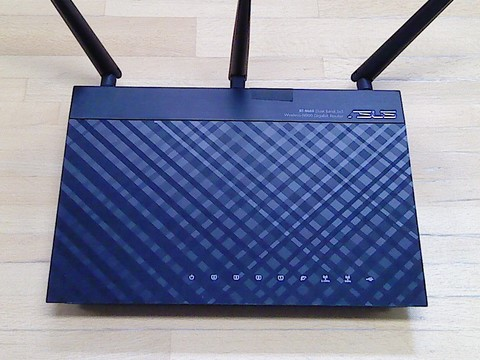
\includegraphics[width=0.35\textwidth]{pics-system/sys-router-front.jpg} &
~ &
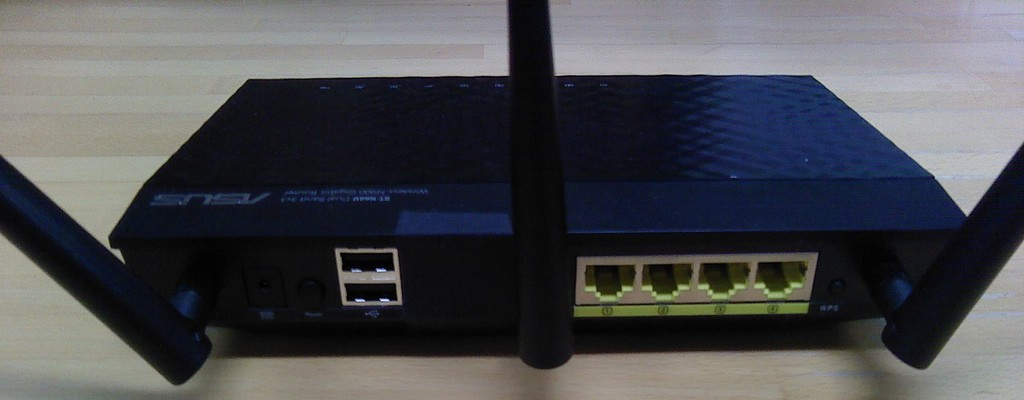
\includegraphics[width=0.45\textwidth]{pics-system/sys-router-back.jpg} \\
\end{tabular}
\end{center}

Changing the administrator login/password (top section):
\begin{center}
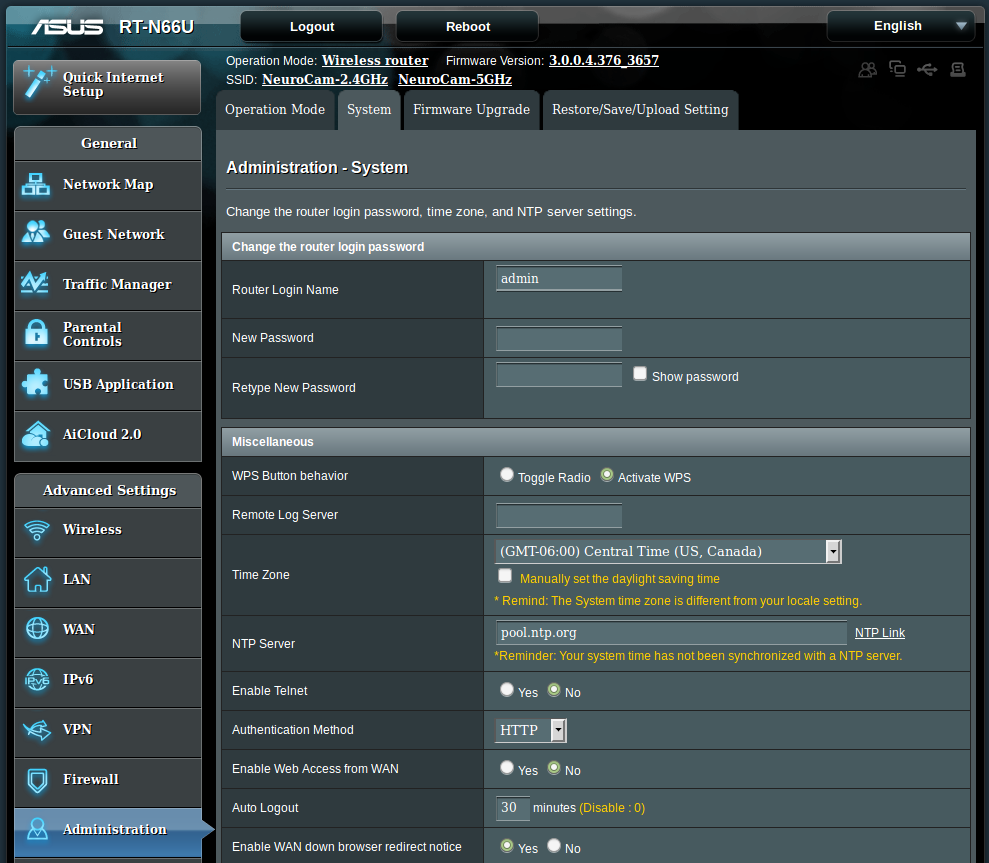
\includegraphics[width=0.7\textwidth]
{pics-router/asus-n66u-admin-pw.png}
\end{center}

% Force a page break.
\clearpage
Setting the wireless network name (``SSID'') and password (``pre-shared 
key''):
\begin{center}
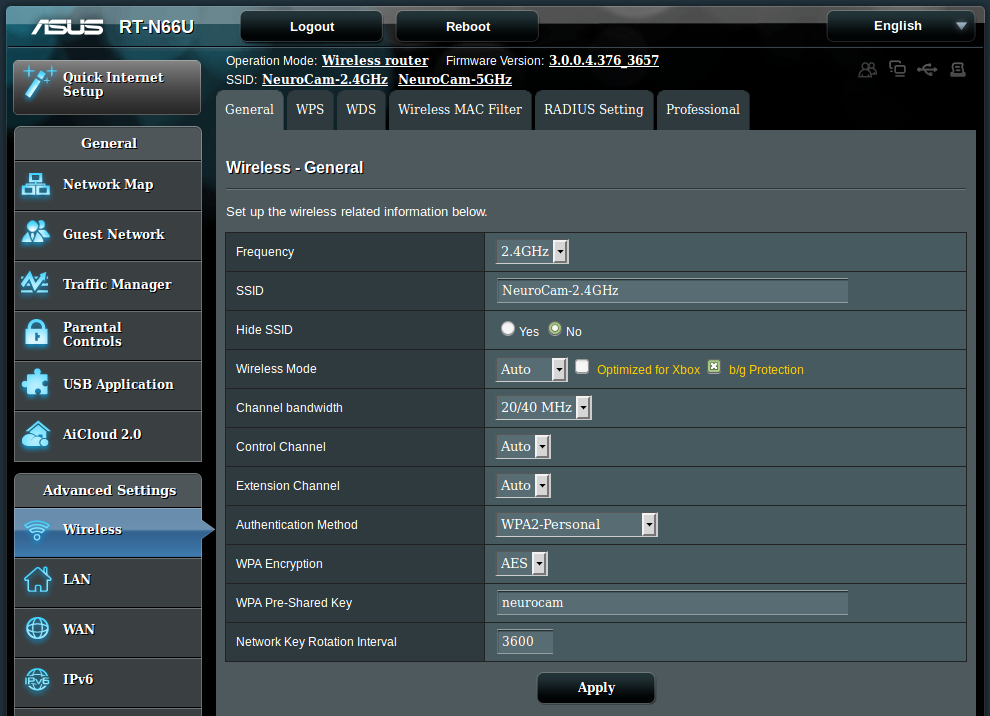
\includegraphics[width=0.7\textwidth]
{pics-router/asus-n66u-ssid.png}
\end{center}

Changing the MAC filter to whitelist mode (``accept the specified 
addresses''), and adding addresses:
\begin{center}
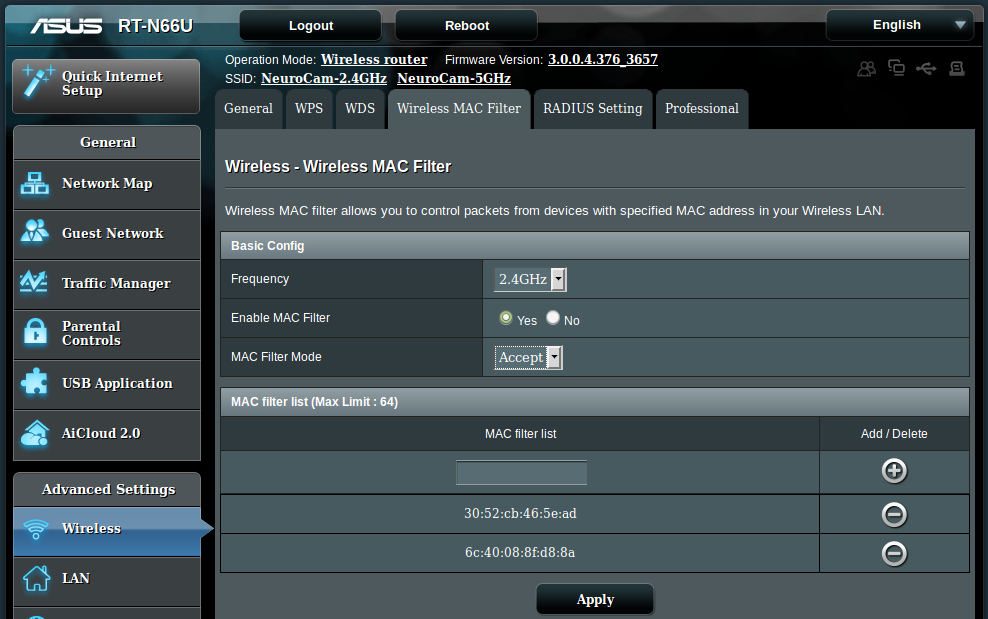
\includegraphics[width=0.7\textwidth]
{pics-router/asus-n66u-macfilter.png}
\end{center}

% Force a page break.
\clearpage
Assigning static IP addresses to specific machines:
\begin{center}
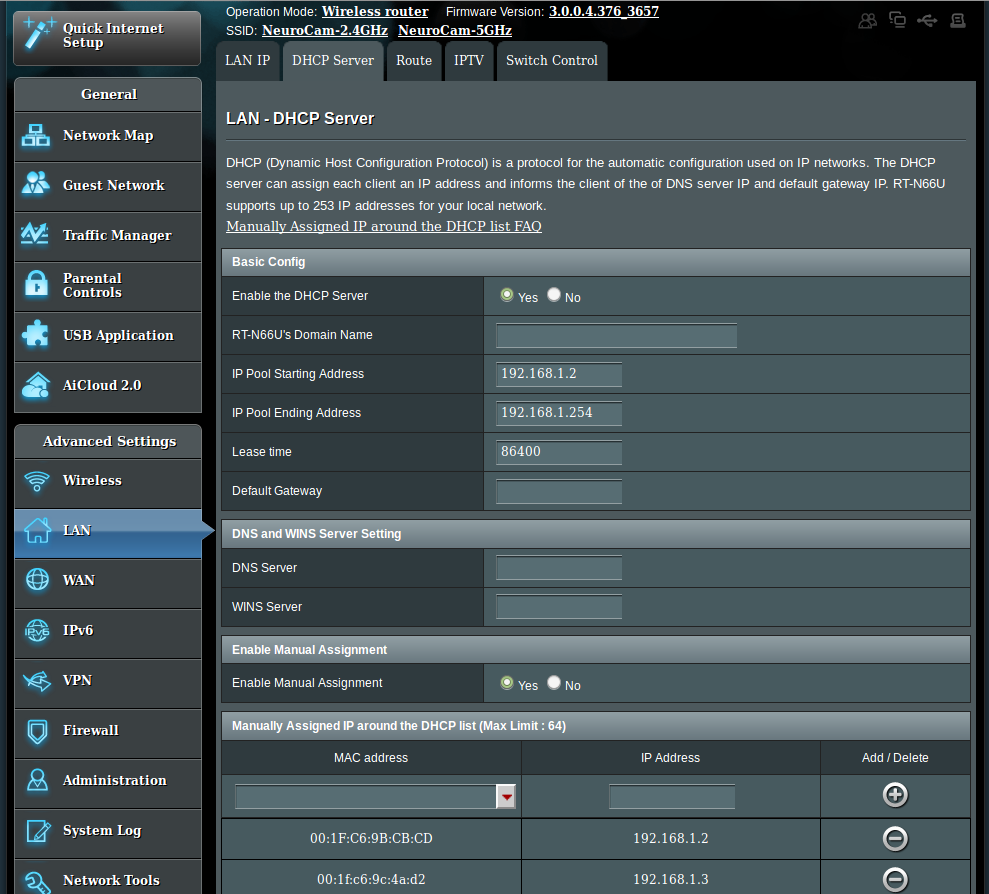
\includegraphics[width=0.7\textwidth]
{pics-router/asus-n66u-static.png}
\end{center}

%
%
\clearpage
\section{Installing OpenWrt}

\fixme{This hasn't been implemented, so no documentation for it.}

{\itshape The idea is to provide scripts that automatically configure and
compile the ``\verb+OpenWrt+'' open--source firmware. This lets us lock down
any features we don't want active, force an appropriate filtering mode, and
disable the web interface (which is one of the main security holes).

Implementing this is deferred, as it will be time--consuming.}

%
% This is the end of the file.

% NeuroCam manual - GPIO/Synch Boxes
% Written by Christopher Thomas.
% Copyright (c) 2021 by Vanderbilt University. This work is released under
% the Creative Commons Attribution-ShareAlike 4.0 International License.

\chapter{GPIO and Synch Box}
\label{gpio}

The GPIO-and-synch box provides TTL-level inputs via a rectangular connector
and TTL-level synchronization outputs via BNC connectors. Changes to inputs
are reported to the NeuroCam computer via USB cable.

During normal operation of the NeuroCam system, the following functions are
performed:
\begin{itemize}
\item The synchronization lines are strobed high for 20~ms every 10 seconds,
with changes in the outputs recorded in session log files.
\item Changes to TTL inputs are recorded in session log files.
\item Low-to-high transitions on input bits 7 and 6 cause the NeuroCam to
start and stop recording a session, respectively. There is a ``dead time''
of 10 seconds between successive commands being recognized.
\end{itemize}

The front panel and interior of a GPIO-and-synch box are shown below:

\begin{center}
% The exterior image is 800x600, the interior is 600x600.
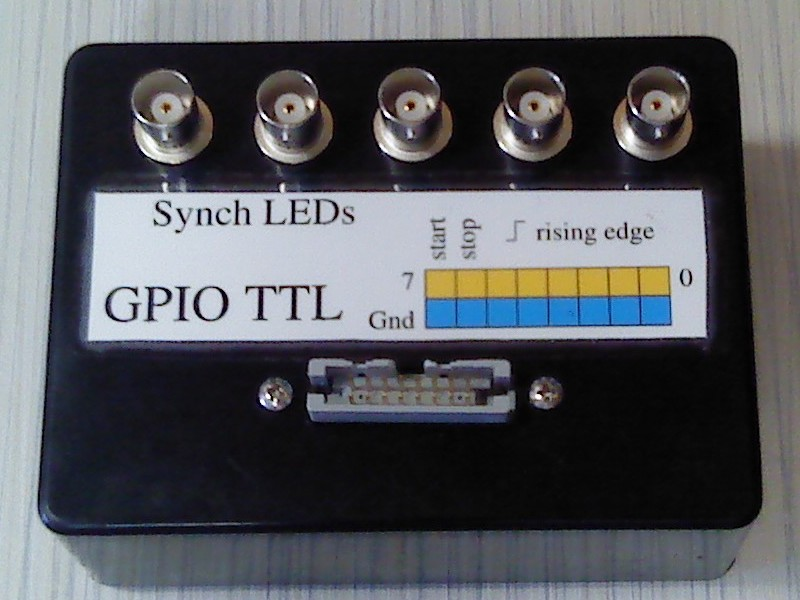
\includegraphics[height=2in]{pics-gpio/gpio-closed.jpg}
\hspace{1in}
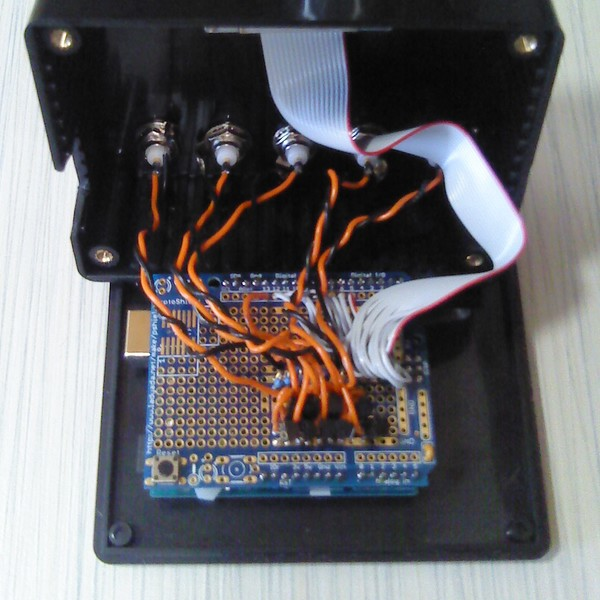
\includegraphics[height=2in]{pics-gpio/gpio-open.jpg}
\end{center}

\clearpage
The parts needed for a GPIO-and-synch box are as follows:

\begin{tabular}{llll}\hline
Qty & Description & Manuf. p/n & Digikey p/n \\
\hline
%
1 & Arduino Uno rev3 & A000066 & 1050-1024-ND \\
1 & Arduino prototyping shield kit & 2077 & 1528-1207-ND \\
9 & NFET TO-92 & BS170 & BS170-ND \\
3 & resistor 4.75 kohm 0.25w & MFR-25FBF52-4K75 & 4.75KXBK-ND \\
7 & resistor 475 ohm 0.25w & MFR-25FBF52-475R & 475XBK-ND \\
5 & BNC jack panel mount & 31-221-RFX & ARFX1064-ND \\
1 & box abs 4.3x3.2x1.7 & 1591SBK & HM121-ND \\
1 & conn 16 pin female to ribbon & M1YXK-1636J & M1YXK-1636J-ND \\
2 & machine screw 4-40 0.5in ss & 9902 & 36-9902-ND \\
2 & hex nut 4-40 ss & 7248-3 & 36-7248-3-ND \\
4 & machine screw 4-40 0.375in nylon & 9528 & 36-9528-ND \\
4 & hex nut 4-40 nylon & 9605 & 36-9605-ND \\
1 & USB cable male A to male B & 102-1030-BE-00200 & 1175-1089-ND \\
%
\hline
\end{tabular}

\textbf{NOTE:} The prototyping shield kit includes male pin headers,
one female ISP header, two decoupling capacitors, one pushbutton switch,
one red LED, and one green LED, which are required for the GPIO-and-synch
box.

The prototyping shield kit should be assembled per its directions. There are
several important things to keep in mind:
\begin{itemize}
%
\item The pin headers (including ISP header) should be plugged into an
Arduino Uno, with the prototyping shield board friction-seated on the header
pins, prior to soldering. This guarantees proper mechanical alignment of the
headers.
%
Do not use the long-tail female ``stacking'' headers for I/O pins. These
do not mate properly with the Arduino Uno. The only female header used is
for the ISP header connection.
%
\item The two decoupling capacitors should be soldered in their marked
positions on the board.
%
\item Only one of the two provided switches is used. This is soldered to
the ``reset switch'' location indicated on the board.
%
\item The red and green 3mm LEDs are not soldered to the prototyping board.
They are used for strobe and power lights on the front panel of the
GPIO-and-synch box if such lights are desired. They mount in 1/8" holes,
and should be secured in place using epoxy on their rear sides.
%
\end{itemize}

\clearpage
The following circuit should be built on the prototyping shield:

\begin{center}
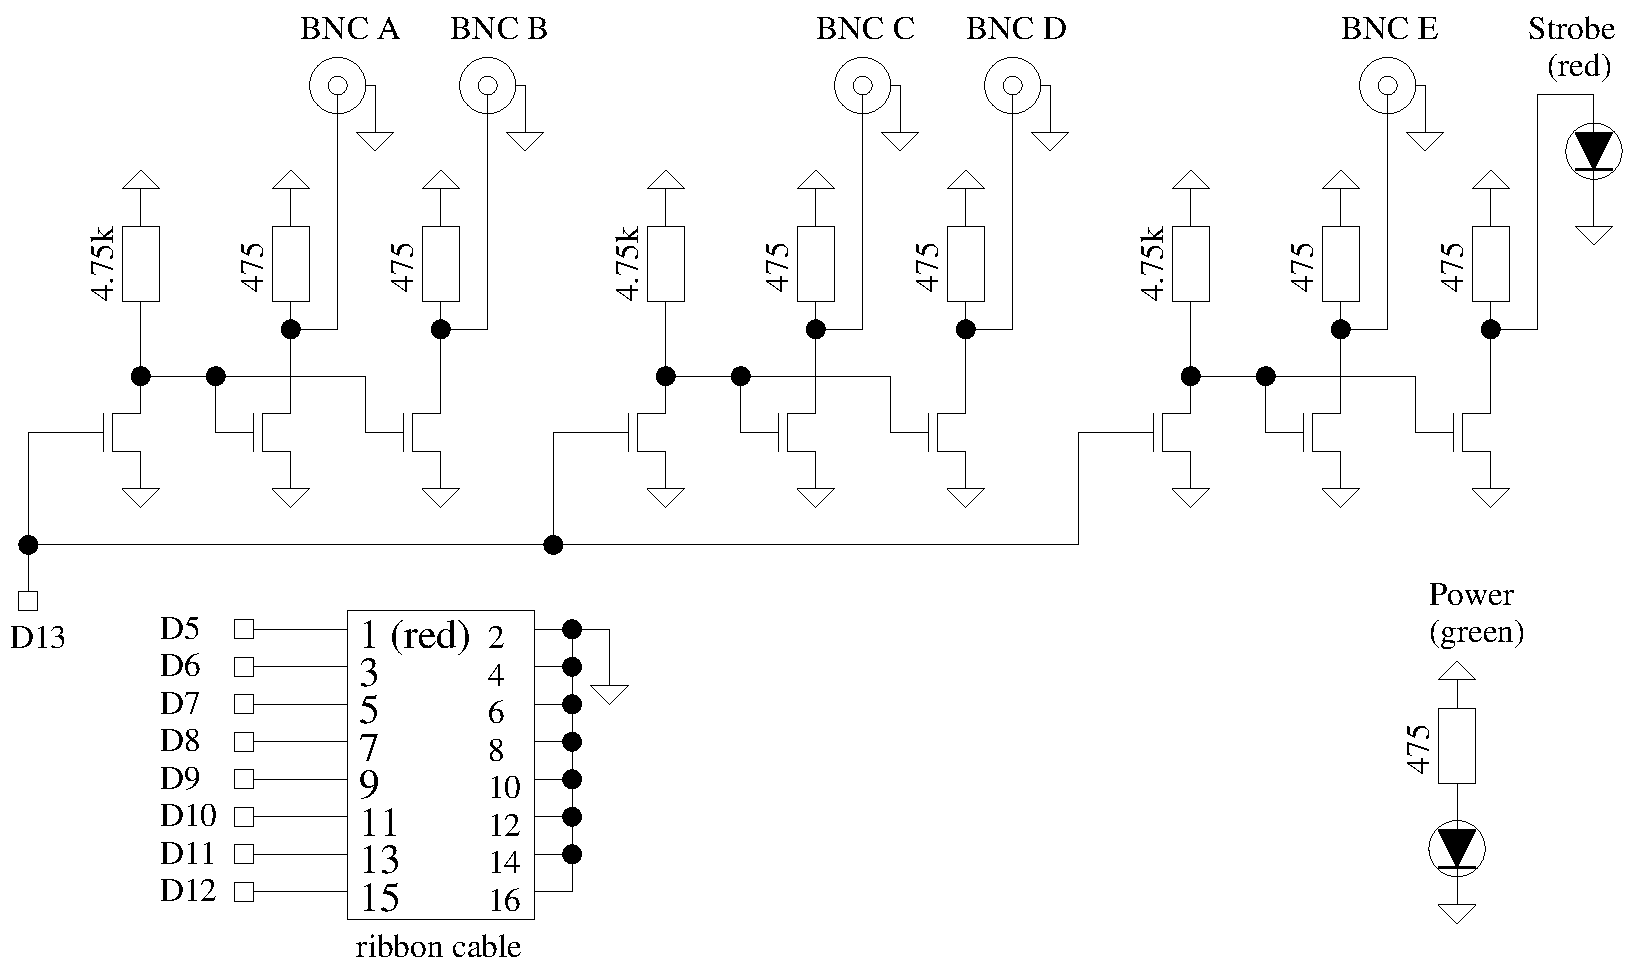
\includegraphics[width=0.9\textwidth]{schematics/gpio-dev-schem.pdf}
\end{center}

A mechanical drawing of the front panel is as follows:

\begin{center}
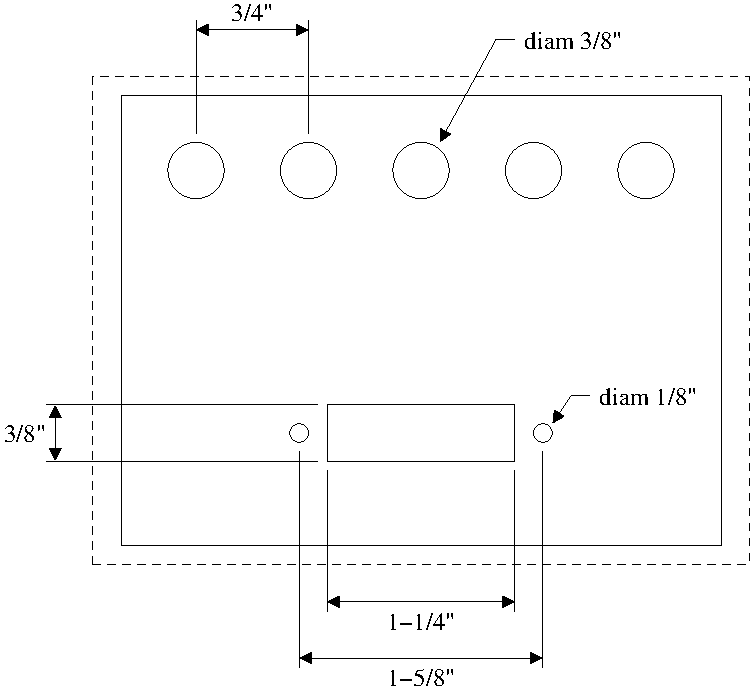
\includegraphics[height=3in]{drawings/gpio-dev-front-mech.pdf}
\end{center}

The rear panel should have mounting holes compatible with the Arduino Uno
(1/8", countersunk).

%
% This is the end of the file.

% NeuroCam manual - Cameras
% Written by Christopher Thomas.
% Copyright (c) 2021 by Vanderbilt University. This work is released under
% the Creative Commons Attribution-ShareAlike 4.0 International License.

\chapter{Cameras}
\label{cameras}

\section*{Camera Selection}

The NeuroCam system is compatible with any UVC-compliant USB camera capable
of producing MJPEG output. That said, there are several additional qualities
that cameras \textit{should} possess:

\begin{itemize}
\item The camera should support 1280x720 or better resolution at 30~fps.
\item The camera should either not have an infrared filter or should have an
infrared filter than can be easily removed (not bonded to the sensor die).
\item The camera should request only the USB bandwidth it needs, rather than
attempting to request all USB bandwidth.
\end{itemize}

The Logitech C920 webcam satisfies these requirements and was used for the
prototype systems. Infrared filter removal with this camera is described in
Chapter \ref{c920}.

\section*{Infrared LED Mounting}

An infrared LED is bonded to each camera to allow individual camera feeds
to be synchronized with high accuracy via strobe flashes. This LED should
not obstruct the scene, but should still be within the camera's field of
view for all video resolutions of interest.

The recommended procedure for mounting LEDs is to set up a video feed from
the camera, apply cyanoacrylate glue (``super glue'') to the camera case,
hold the LED mounting rod in position until the glue sets (using the video
feed to guide placement), and then to apply two-part epoxy for a more
permanent bond.

For the Logitech C920, positioning the LED in the upper left corner of the
field of view when using a 4:3 resolution guarantees that it is visible in
all video modes (4:3 and 16:9).

The parts needed to add LEDs to each camera are as follows:

\begin{tabular}{llll}\hline
Qty & Description & Manuf. p/n & Digikey p/n \\
\hline
1 & NIR LED 940nm & SLED-56-16639 & SLED-56-16639-ND \\
1 & BNC female to wire & BU-P4969 & 314-1190-ND \\
\hline
\end{tabular}

Mechanical details for mounting LEDs to Logitech C920 cameras are shown
below:

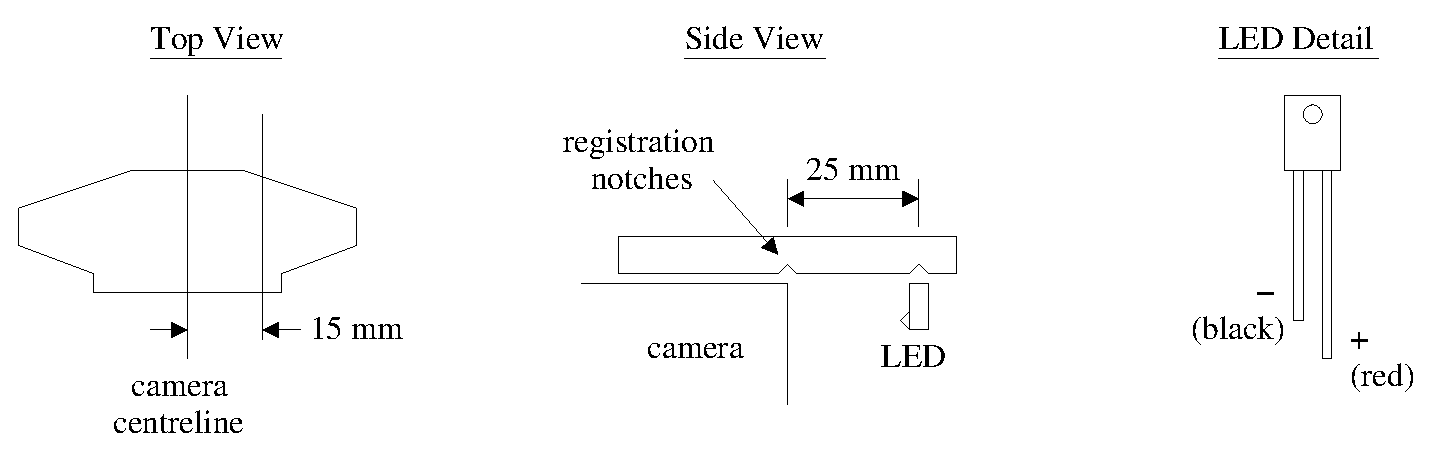
\includegraphics[width=0.9\textwidth]{figs/maint-led-920.pdf}

The result is shown below:
\begin{center}
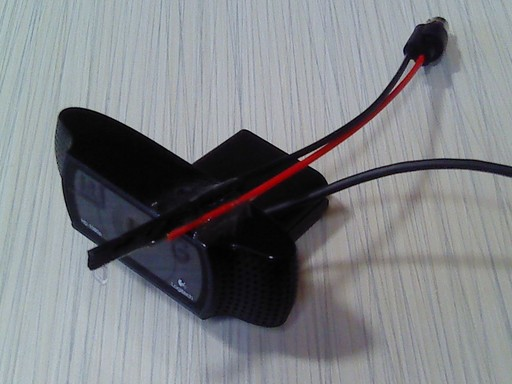
\includegraphics[height=3in]{pics-cam/c920-led.jpg}
\end{center}

%
% This is the end of the file.

% NOTE - c920 IR modifications have been split off to their own document.

% Part 3: Developer guide.

\clearpage
\pagestyle{empty}
\part{Modifying the NeuroCam Software}
\pagestyle{plain}

% NeuroCam manual - Development Computer
% Written by Christopher Thomas.
% Copyright (c) 2021 by Vanderbilt University. This work is released under
% the Creative Commons Attribution-ShareAlike 4.0 International License.

\chapter{Development Computer}
\label{devmachine}

The NeuroCam development environment is an x86-architecture computer running
the Linux Mint operating system, with the NeuroCam software and its required
support packages installed.

Hardware specifications are not critical, but if more than two cameras are to
be tested on a development machine, hardware performance comparable to the 
NeuroCam computer described in Chapter \ref{machine} will be needed.

To build a new NeuroCam development computer, you will need the following:
\begin{itemize}
%
\item A suitable computer.
\item A USB stick containing the Linux Mint 18.1 installer.
\item A USB stick containing the NeuroCam installer and the NeuroCam
development environment.
%
\end{itemize}

Making a NeuroCam development environment USB stick is described in Section
\ref{devmachine-usb}. Making a NeuroCAM install USB stick is described in
Section \ref{machine-usb}. Both of these may be placed on the same USB stick.

Making a Linux Mint install USB stick is described in Section
\ref{machine-usbmint}.

%
%
\section{First-Time Installation}

This is a variation of the procedure used for NeuroCam computers. There are
important differences, so be sure to check the steps closely.

\fixme{This uses the NeuroCam computer install scripts, which require the
username ``neurocam-admin''. Dedicated dev scripts would relax that
requirement.}

To install Linux and the NeuroCam software (but not the development
environment):
\begin{itemize}
%
\item Connect the machine to a keyboard, a mouse, and a monitor.
\item With the machine unpowered, plug in the Mint 18.1 USB stick.
\item Turn on the machine.
\item Get to the BIOS menu by holding the appropriate key during boot
(usually F2).
\item Turn UEFI off. This may be called ``Windows compatibility''.
\item Edit the boot order, moving the USB stick to the top.
\item Hit F10 to save and exit.
%
\item (The machine should now show the Linux boot menu.)
\item From the Linux boot menu, pick ``start in compatibility mode''.
\item From the GUI, open a terminal window.
\item Type ``\verb+sudo bash+'' to get a root session.
\item Type ``\verb+fdisk /dev/sda+'' to partition the drive.
\item Delete any existing partitions. The normally won't be any.
\item Create a 50 gigabyte partition (for the OS), an 8 gigabyte partition
(for swap space), and a third partition (for data).
\item Set the OS and data partitions to type 83 (Linux; this may be set
already by default). Set the swap partition to type 82 (Linux swap).
\item Set the ``bootable'' flag on the OS partition.
\item Save and exit \verb+fdisk+.
\item Type ``\verb+mke2fs -j /dev/sda1+'' and
``\verb+mke2fs -j -m 0 /dev/sda3+'' to create filesystems on the OS and
data partitions, respectively.
\item Type ``\verb+mkswap /dev/sda2+'' to initialize the swap partition.
\item Type ``\verb+exit+'' twice to leave the root shell and the terminal
window.
%
\item Click ``Install Linux Mint''.
\item Do not set up networks.
\item Do not install proprietary software.
\item Select ``Something Else'' for the target partition.
\item Doubleclick ``\verb+/dev/sda1+'', select ``use as ext3 journaling
filesystem'', check ``format'', and select mount point ``/''.
\item Doubleclick ``\verb+/dev/sda2+'', and select ``use as swap area''.
\item Doubleclick ``\verb+/dev/sda3+'', select ``use as ext3 journaling
filesystem'', check ``format'', and select mount point ``/data''.
\item Click ``Install Now''.
\item Select time zone and keyboard type.
\item For ``Your Name'', enter ``NeuroCam Developer''. Enter any desired
name for ``Your Computer's Name'' (allowable characters are lower--case 
letters, numbers, and hyphen; no whitespace, capitals, or punctuation).
For ``Pick a User Name'', enter ``\verb+neurocam-admin+''. For the password,
enter ``\verb+neurocam+''.
\par
\textbf{This password is easily guessed, and so should be changed when
setup is completed.} The procedure for changing passwords is described in
Section \ref{machine-password}.
\item Check ``require password to log in''.
\item Begin the install.
\item When the installation finishes, click ``restart now''.
\item Remove the USB stick when the system reboots.
%
\item (The system should boot to the Linux Mint login screen.)
\item Log in as ``\verb+neurocam-admin+'' with the password
``\verb+neurocam+''.
\par
\textbf{NOTE:} If the system does not let you log in with the credentials
supplied above, see Section \ref{machine-password} for the password reset
method.
%
\item (You should now be logged in as ``\verb+neurocam-admin+'' on a graphical
desktop.)
\item Click the terminal icon in the hotbar or start menu to get a terminal
window with a command shell.
\item In the terminal window, type ``\verb+sudo bash+'' to get a root shell.
Enter ``\verb+neurocam+'' as the \verb+sudo+ password.
\item Type ``\verb+passwd+'' to reset the \verb+root+ account's password.
Set it to ``\verb+administrator+''.
\par
\textbf{This password is easily guessed, and so should be changed when
setup is completed.} The procedure for changing passwords is described in
Section \ref{machine-password}.
\item Type ``\verb+exit+'' to leave the root shell.
\item Type ``\verb+exit+'' again to leave the command shell, closing the
terminal window.
\item Click on the ``log out'' icon in the start menu.
%
\item Press \verb+ctrl-alt-F6+ to get to a text console (if using a Mac
keyboard, \verb+ctrl-option-function-F6+).
\item Log in as ``\verb+root+'' with the password ``\verb+administrator+''.
\item Plug the development computer into an internet jack.
\item Wait 10 seconds.
\item Type ``\verb+ifconfig+'' to get network interface information. Wired
ethernet is the entry with a device name starting with ``\verb+e+'' (usually
``\verb+eth+'', ``\verb+eno+'', ``\verb+enp+'', or similar).
\item When network handshaking has finished, there will be an
``\verb+inet addr+'' field with an IP address assigned. This address will
\textbf{not} start with \verb+127+ (\verb+127.x.x.x+ is the loopback address).
\item Your institution's network may require network cards' MAC addresses
to be registered before allowing connections. To find the network card's MAC
address, look for a field named ``\verb+HWaddr+''. Write this down.
\item Type ``\verb+ping 8.8.8.8+'' to check internet connectivity. A response
of ``\verb+64 bytes from 8.8.8.8+'' means that the internet is visible.
\item Type ``\verb+mkdir /usb+'' to create a manual mount point for the USB
stick. This only needs to be done once.
\item Make sure no other USB sticks are in the machine, and insert a
NeuroCam update USB stick.
\item Type ``\verb+mount -t auto -o exec /dev/sdb1 /usb+'' to manually mount
the USB stick and to allow scripts to be run from the stick.
\item Type ``\verb+/usb/neurocam-install/scripts/do-install.sh+'' to perform
first-time NeuroCam software installation. This will take a while.
\par
\textbf{NOTE:} This should skip most confirmation steps, but may still ask for
user input. Default settings should always be acceptable.
\item Once this has finished, type ``\verb+shutdown -r now+'' to reboot.
\item Remove the USB stick when the system reboots.
%
\end{itemize}

To install the development environment:
\begin{itemize}
%
\item Allow the machine to boot to the graphical login screen as normal.
\par
(To switch from the text logon screen to the graphical screen, press
\verb+ctrl-alt-F8+; on a Mac keyboard, \verb+ctrl-option-function-F8+.)
\item Log in as ``\verb+neurocam-admin+''.
\item Make sure no other USB sticks are in the machine, and insert a NeuroCam
development USB stick. Close the file browser popup window, if any.
\item Click the terminal icon in the hotbar or start menu to get a terminal
window with a command shell.
\item Navigate to the directory you wish to use as the development tree root.
You can create a new directory with ``\verb+mkdir ~/(directory)+'' and move
to it with ``\verb+cd ~/(directory)+''. Type ``\verb+pwd+'' to check that you
are in the desired location.
\item Type ``\verb+tar -xvf /media/neurocam-admin/(label)/neurocam/dev/*.tar+''.
\par
This refers Mint's automatic mount point for the USB stick, with 
``\verb+(label)+'' replaced with the stick's volume label (or serial number if
there is no volume label). You can use ``tab completion'' to avoid having to
type this: if only one USB stick is plugged in, 
``\verb+/media/neurocam-admin/(tab)+'' will automatically expand to the
correct mount point name when the \verb+tab+ key is pressed.
\item When the ``\verb+tar+'' command has finished extracting files, type
``\verb+ls+'' to check that the development tree's subdirectories are in 
place.
\item Type ``\verb+umount /media/neurocam-admin/(label)+'' to unmount the
USB stick for safe removal.
%
\end{itemize}

%
%
\section{Updating the Development Machine}

Linux will usually update itself automatically, but doing this manually is
also acceptable. The NeuroCam software and the NeuroCam development code
will have to be updated manually.

Updating Linux Mint requires an internet connection. Updating the NeuroCam
software and development code do not.

To update Linux Mint:
\begin{itemize}
%
\item (Turn on the machine and allow it to boot per normal.)
\item Press \verb+ctrl-alt-F6+ to get to a text console.
\item Log in as ``\verb+root+''.
\item Type ``\verb+ping 8.8.8.8+'' to check internet connectivity. A response
of ``\verb+64 bytes from 8.8.8.8+'' means that the internet is visible.
\item Type ``\verb+~/neurocam-scripts/do-mintupdate.sh+''. This may take a
while, depending on how many packages need to be updated.
\par
\textbf{NOTE:} This should skip most confirmation steps, but may still ask for
user input. Default settings should always be acceptable.
\item Type ``\verb+exit+'' to log out.
\item Press \verb+ctrl-alt-F8+ to return to the graphical login screen.
\end{itemize}

To update the NeuroCam software:
\begin{itemize}
%
\item (Turn on the machine and allow it to boot per normal.)
\item Press \verb+ctrl-alt-F6+ to get to a text console.
\item Log in as ``\verb+root+''.
\item Make sure no other USB sticks are in the machine, and insert a
NeuroCam update USB stick.
\item Wait five seconds, then type ``\verb+mount /usb+''.
\item Type ``\verb+~/neurocam-scripts/do-update.sh+''.
\item Once this has finished, type ``\verb+shutdown -r now+'' to reboot.
This will force a full restart of the NeuroCam software.
\item Remove the USB stick when the system reboots.
%
\end{itemize}

To update the NeuroCam development environment:
\begin{itemize}
\item (Turn on the machine and allow it to boot to the graphical login
screen as normal.)
\item Log in as ``\verb+neurocam-admin+''.
\item Make sure no other USB sticks are in the machine, and insert a NeuroCam
development USB stick. Close the file browser popup window, if any.
\item Click the terminal icon in the hotbar or start menu to get a terminal
window with a command shell.
\item Navigate to the directory you use as the development tree root.
Type ``\verb+pwd+'' to check that you are in the desired location.
\item \textbf{Make sure that you have backed up any changed files.}
Reinstalling the development tree will overwrite any existing files that are
present.
\item Type ``\verb+tar -xvf /media/neurocam-admin/(label)/neurocam/dev/*.tar+''.
\item When the ``\verb+tar+'' command has finished extracting files, type
``\verb+ls+'' to check that the development tree's subdirectories are in 
place.
\item Type ``\verb+umount /media/neurocam-admin/(label)+'' to unmount the
USB stick for safe removal.
\end{itemize}

%
%
\section{Making New Development USB Sticks}
\label{devmachine-usb}

The NeuroCam development environment can be added to any USB stick. This
does not interfere with existing data; the software is placed in a new
directory called ``\verb+neurocam-dev+''.

To add the install and update software to an already-formatted USB stick:
\begin{itemize}
\item On a NeuroCam development machine, open a terminal window.
\item Navigate to the NeuroCam development directory.
\item Make sure no other USB sticks are in the machine, and insert a USB
stick to turn into a NeuroCam update USB stick.
\item Type ``\verb+install/scripts/make-devkey.sh+''.
\item Wait until the script has finished.
\item Type ``\verb+umount /media/neurocam-admin/(label)+'' to unmount the
USB stick for safe removal.
\end{itemize}

%
% This is the end of the file.

% NeuroCam manual - Network Communication Between Components
% Written by Christopher Thomas.
% Copyright (c) 2021 by Vanderbilt University. This work is released under
% the Creative Commons Attribution-ShareAlike 4.0 International License.

\chapter{Network Communication Between Components}
\label{netcomm}

\section{Overview}

The NeuroCam software consists of several components that interact via UDP 
network messages. A diagram is shown below:

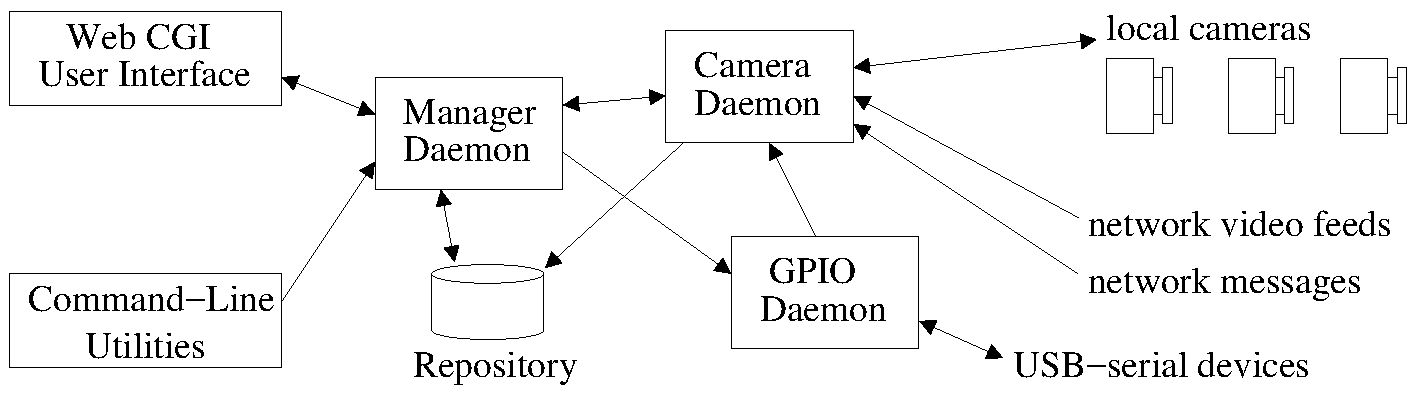
\includegraphics[width=0.9\columnwidth]{figs/dev-netcomm.pdf}

The camera daemon collects local camera video and collects video frames and 
UDP messages from external sources (using the handshaking protocol 
described in Chapter \ref{handshake}).
The GPIO daemon monitors USB-attached serial tty devices, talks to ones
that recognize its handshaking protocol, and reports changes to their state.
The manager daemon coordinates activities at the top level, and a web CGI 
script processes user requests and turns these into commands that are sent 
to the manager daemon.

This architecture was chosen for modularity/compartmentalization. In 
particular, the CGI web interface may be replaced with any other interface
that can talk to the manager daemon over UDP.

% FIXME - Force a page break.
\clearpage
The ports reserved for these communications are defined in the
``\verb+network+'' library file. A summary is below:

\begin{tabular}{ccp{0.7\columnwidth}} \hline
Port & Used By & Purpose \\ \hline
%
7xxx & other &
Default port address range for the network library. Chosen to not conflict
with any other port ranges. \\
\hline
8080 & \verb+fakeunity+ &
Port on which the fake game utility offers its video feed. \\
8090 & (camera) \verb+daemon+ &
Port on which the camera daemon offers the monitoring video feed. \\
8888 & game, \verb+fakeunity+ &
Broadcasts asking for external information sources (videos, UDP messages)
are made to this port. Anything with information to offer should listen 
at this address. \\
\hline
9xxx & (camera) \verb+daemon+ &
Port range reserved for the camera daemon. \\
9998 & (camera) \verb+daemon+ &
Port on which the camera daemon tells itself that it's finished assembling 
a monitoring frame. \\
9999 & (camera) \verb+daemon+ &
Port on which the camera daemon listens for commands. \\
\hline
10xxx & \verb+manager+ &
Port range reserved for the manager daemon. \\
10999 & \verb+manager+ &
Port on which the manager daemon listens for commands/queries. \\
\hline
11xxx & \verb+fakeunity+ &
Port address range reserved for the fake game utility. This is chosen to not 
conflict with any other port ranges. This has to be set to something, because 
the network library can reserve access to ports when used and these will not 
be released until the fake game utility terminates. \\
\hline
12xxx & \verb+cgi+ web script &
Port address range reserved for the CGI script. \\
\hline
13xxx & \verb+mjpeg+ library &
Port range reserved for internal communication by the multithreaded version 
of the video serving function. Multiple instances of that function will 
use overlapping ranges and fight over ports, so the single-threaded version 
should be used when possible. \\
\hline
14000 & \verb+gpio+ &
Port on which the GPIO daemon listens for commands/queries. \\
%
\hline
\end{tabular}

\section{Manager Daemon}

The manager daemon is responsible for starting and stopping the camera daemon,
for ensuring that the GPIO daemon is running, and for performing 
post-processing and other repository manipulations.

The manager daemon listens for UDP packets on port 10999. Commands are
plain text strings.

Multiple commands may be issued in sequence (the manager will accept and
make note of new commands while processing previous commands). Some commands,
like status queries, will be executed immediately even if other tasks are
ongoing; others, like post-processing tasks, will be queued in sequence.

\textbf{NOTE:} Directory paths and filenames are \textbf{not checked}. A
malicious user could abuse this, so it is \textbf{strongly recommended} that 
all such names be script-generated and not based on user input.

Status query command:
\begin{itemize}
\item ``\verb+what is your status reply to port NNNN+''
\end{itemize}

% FIXME - Force a page break.
\clearpage
Status responses:
\begin{itemize}
\item ``\verb+idle+''
\item ``\verb+running cameras+''
%
\item ``\verb+busy (doing what) (progress string)+''

The progress string is optional, and is always in parentheses if present.
The operation specifier (also optional but usually present) is one of the
following:
\begin{itemize}
\item ``\verb+synchronizing timestamps+''
\item ``\verb+compositing+''
\item ``\verb+transcoding+''
\item ``\verb+archiving+''
\item ``\verb+calculating sizes+''
\item ``\verb+removing post-processed files+''
\item ``\verb+removing session folder+''
\item ``\verb+copying session folder+''
\item ``\verb+synchronizing disks+''
\item ``\verb+generating preview+''
\item ``\verb+auto-adjusting cameras+''
\end{itemize}
%
\end{itemize}

Diagnostics commands:
\begin{itemize}
\item ``\verb+debug version to port NNNN+''

The response to this is a version string.

\item ``\verb+debug report to port NNNN+''

The response to this is one or more messages describing the manager's internal
state and the last command processed.
\end{itemize}

Session commands:

\begin{itemize}
\item ``\verb+start cameras repository=(dir) config=(file)+''

Specifying ``\verb+auto+'' for the repository or config file tells the
manager to choose its own values for those parameters. An automatic
repository name will be based on a timestamp.

A copy of the configuration file will be placed in the new session folder.

\item ``\verb+stop cameras+''
\item ``\verb+shut down+''
\end{itemize}

% FIXME - Force a page break.
\clearpage
Monitoring commands (used only while recording):
\begin{itemize}
\item ``\verb+feed (subdir name)+''

The default feed is ``\verb+Monitor+'', which is a stitched-together tiling
of all video feeds. Other feed names just copy one stream's frames directly.
\end{itemize}

Video configuration commands (used only while not recording):
\begin{itemize}
\item ``\verb+snapshot config=(file) outdir=(dir)+''

This acquires frames from all local cameras and all non-local video streams,
saving the results in the ``\verb+auxfiles+'' directory.

\item
``\verb+autocamadjust config=(file) size=(resolution wanted) rate=(fps wanted)+''

This walks through all cameras, adjusting size and exposure settings until
the desired frame rate is obtained. First exposure time is reduced, and if
that fails to produce the desired frame rate size is reduced and the process
repeats. This is very time-consuming.
\end{itemize}

Post-processing commands (used only while not recording):
\begin{itemize}
\item ``\verb+timeshift repository=(dir)+''

This adjusts each video stream's timestamps so that LED flashes are 
synchronized. Only produces valid results if flashes are present.

This creates a modified log file (``\verb+logfile-timed.txt+'') with 
altered timestamps.

\item ``\verb+composite repository=(dir)+''

Assembles a ``Composite'' video feed. This stitches together frames from all
other video feeds, in the same manner as the ``Monitor'' feed, but does so at
higher resolution, with no dropped frames, and with a visible timestamp 
annotation.

This creates a modified log file (``\verb+logfile-composited.txt+'') with
frame events for the ``\verb+Composited+'' video feed inserted.

\item 
``\verb+transcode repository=(dir) stream=(subdir name) output=(file w/o suffix)+''

This assembles frames from one video feed directory into a playable compressed
video file (typically ``\verb+.mp4+'' format).

\textbf{NOTE:} because this performs lossy compression on what was already 
lossy-encoded MJPEG data, the image quality of frames suffers. Compressed 
video files are intended for user preview purposes, not automated processing.

\item ``\verb+archive rootdir=(dir) output=(file without suffix)+''

This creates a ``\verb+.tar+'' archive with the contents of a directory
(typically a session folder). This is intended to allow convenient web 
download of a folder's contents.

\item ``\verb+unprocess repository=(dir)+''

This removes all post-processing files associated with a directory (which
should be a session folder). This includes modified/annotated log files,
compressed video streams, the ``Composite'' video stream's folder, and any
``\verb+.tar+'' archive created of this directory.

\item ``\verb+cancel processing+''

This halts post-processing. The command in progress is killed, remaining
queued commands are purged, and an ``\verb+unprocess+'' command is
automatically queued for execution.
%
\end{itemize}

Repository manipulation commands (used only while not recording):
\begin{itemize}
\item ``\verb+metadata rootdir=(dir)+''

This refreshes metadata for all session folders within a given repository
root directory. This can take quite a while, as updating a changed session 
folder potentially involves checking metadata for millions of files.

\item ``\verb+copy source=(dir) dest=(dir)+''

This duplicates a directory tree (which is intended to be a session folder). 
The original is left intact; for a ``move'' operation, issue a 
``\verb+delete+'' command following this one.

\item ``\verb+delete repository=(dir)+''

This removes a directory tree (which is intended to be a session folder).

\item ``\verb+disksynch+''

This issues a ``\verb+sync+'' command, committing changes to disk. This is
intended to allow safe removal of USB drives, which can take substantial
amounts of time to commit changes.
%
\end{itemize}

\section{Camera Daemon}

\fixme{Content goes here.}

\section{GPIO Daemon}

\fixme{Content goes here.}

Talk about handshaking with GPIO devices over USB-serial.

\section{Web Interface Notes}

\fixme{Content goes here.}

Talk about where scratch files go, what the default directories are,
and the paradigm the CGI script uses.

\fixme{Stopped here.}

%
% This is the end of the file.

% NeuroCam manual - Data Structures
% Written by Christopher Thomas.
% Copyright (c) 2021 by Vanderbilt University. This work is released under
% the Creative Commons Attribution-ShareAlike 4.0 International License.

\chapter{Data Structures}
\label{structs}

\section{Camera Configuration Structure}

\fixme{Content goes here.}

\section{Network Entity Configuration Structure}

\fixme{Content goes here.}

\section{Session Configuration Structure}

\fixme{Content goes here.}

\section{Networking Information Structure}

\fixme{Content goes here.}

\section{Configuration File Format}

\fixme{Content goes here.}

%
% This is the end of the file.

% NeuroCam manual - Library Functions
% Written by Christopher Thomas.
% Copyright (c) 2021 by Vanderbilt University. This work is released under
% the Creative Commons Attribution-ShareAlike 4.0 International License.

\chapter{Library Functions}
\label{funcs}

\fixme{Content goes here.}

This should give an overview of how libraries are split up, and an overview 
of the functions offered by each library.

While the function and variable lists can be more or less the extracted 
declarations and comments, there should be a preamble for each library 
explaining how all of the pieces fit together and are intended to be used.

%
% This is the end of the file.

% NeuroCam manual - Programs
% Written by Christopher Thomas.
% Copyright (c) 2021 by Vanderbilt University. This work is released under
% the Creative Commons Attribution-ShareAlike 4.0 International License.

\chapter{Executables}
\label{progs}

\fixme{Content goes here.}

This should give an overview of the internal architecture of each executable,
and then go on to describe variables and functions in the same manner as with
libraries.

%
% This is the end of the file.


\end{document}

%
% This is the end of the file.
